\documentclass[a4paper, 12pt]{report}
\usepackage{graphicx} % Required for inserting images
\usepackage[T1]{fontenc}
\usepackage[latin1]{inputenc}
\usepackage{graphicx}
\usepackage{titlesec}
\usepackage{xcolor}
\usepackage{amsfonts}
\usepackage{wrapfig}
\usepackage{amssymb}
\usepackage{mathtools}
\usepackage[hidelinks]{hyperref}
\DeclarePairedDelimiter\ceil{\lceil}{\rceil}
\DeclarePairedDelimiter\floor{\lfloor}{\rfloor}

\usepackage{glossaries}
\newtheorem{theorem}{Theorem}
\newtheorem{lemma}{Definition}
\newtheorem{proposition}{Proposition}
\newtheorem{proof}{Proof}
\usepackage{tikz}
\tikzstyle{mybox} = [draw=black, thin, rectangle, rounded corners, inner ysep=5pt, inner xsep=5pt, fill=orange!20]

\usepackage[a4paper, top=2cm , bottom=2cm , right=2cm , left=2cm ]{geometry}

\graphicspath{ {images/} }

\titlespacing{\title}{10pt}{50pt}{50pt}
\titlespacing{\chapter}{0pt}{10pt}{10pt}
\titlespacing{\section}{10pt}{5pt}{10pt}

\title{
    \textbf{  \Huge{  MODELING AND  CONTROL OF\\ 
    CYBER-PHYSICAL SYSTEMS } }\\
    \textit{Lecture notes}
}
\author{Carlo Migliaccio}
\date{AA 2023/2024}

\begin{document}
\maketitle
\tableofcontents

\part{Modeling of Cyber-Physical systems}
\chapter{Introduction}
\section{Some definitions}
\noindent
\textbf{Definition} (Helen Gill, 2006) "Cyber-Physical systems are physical, biological, and engineered systems whose operations are integrated, \textbf{monitored, and/or controlled} by a \textbf{computational core}. Components are \textbf{networked} at every scale. Computing is deeply embedded into every physical component, possibly even into materials. The computational core is an embedded system, usually demands real-time response, and is most often distributed"\\

\noindent Roughly speaking a CPS is a \textbf{collection of devices} that:
\begin{enumerate}
    \setlength\itemsep{-.5em}
    \item compute
    \item inter-communicate
    \item interact with the physical word
\end{enumerate}

\begin{figure}[h]
    \centering
     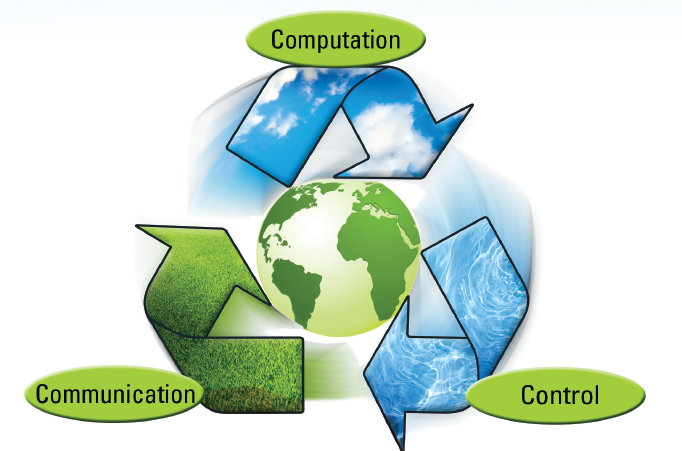
\includegraphics[width=0.6\textwidth]{images/CPS.png}
    \caption{Three Dimensions of CPSs}
    \label{fig:enter-label}
    \end{figure}
    
\noindent 
At this point, we can distinguish in this scenario two layers for CPS: (1) The \textbf{Cyber Layer} which is linked to the computation and communication issues, (2) the \textbf{Physical Layer} deals with the interaction of the devices with the physical word.\\
\vspace{2cm}
%-------------------------------------------------------------

\section{Some examples of CPS}
\noindent
Examples of Cyber-Physical systems could be:
\begin{itemize}
    \item \textbf{Automotive vehicles}: in a car you can find hundreds of sensors, actually we have a computational core, are interconnected in some way (eg. CAN), moreover several feedback-control systems can be find;
    \item \textbf{Teams of mobile robots} that aim to get a target. Robots collaborate to achieve a goal that can be: the exchange of information for example; 
    \item \textbf{Wireless sensor networks} in order to monitor and area (indoor localization without a GPS)
\end{itemize}

%-------------------------------------------------------------
\section{Enabling Technologies and related problems}
\noindent
We can wonder: "How can we deploy CPS?". The answer is by using: 
\begin{enumerate}
    \setlength\itemsep{0em}
    \item \textbf{Embedded systems}: hardware and software integrated within mechanical and electrical systems
    \item \textbf{Sensors and Actuators} for monitoring and control purposes
    \item \textbf{Communication Networks} for example Wireless communication
\end{enumerate}
Despite the \textbf{implementation} it's not too much expensis it raises several issue: at first the \textbf{Vulnerability} which is linked to the \textbf{Safety} of the overall system.

%-------------------------------------------------------------
\section{Mathematical models for CPS}
\noindent
We can modelize a Cyber-Physical System by using: 
\begin{itemize}
      \setlength\itemsep{0em}
    \item \textbf{Basic  Models}: continuos-discrete time LTI systems
    \item \textbf{Hybrid models}: they can describe the interaction between devices and the physical layer including both continuous and discrete events; 
    \item \textbf{Systems under adversarial attacks}: a CPS could be attacked in order to manipulate the exchanged information;
    \item \textbf{Multi-agent systems}: networks of intercommunicating \textit{agents} which may collaborate to reach a \textit{common goal}: \textbf{Consensus}.
\end{itemize}
\subsection*{Hybrid systems}
In order to \textbf{model the presence of physical events} that can change the dynamics, we can consider \textbf{hybrid systems}, also known as  \textbf{switched linear systems}. We can describe them by using the following formalism:
\vspace{1cm}
\begin{large}
    \begin{align*}
    &x(k+1)=A_{q_k}x(k)+B_{q_k}u(k)\\
    &y(k)= C_{q_k}x(k)+D_{q_k}u(k) 
\end{align*}
\end{large}

\vspace{3cm}
for $k=0,1,...$
\begin{itemize}
    \setlength\itemsep{0em}
    \item $x(k)$ is the continuous state
    \item $q_k \in \{1, 2, ..., Q\}$ is the discrete state or {\color{red} mode}, if $q_k \neq q_{k+1}$ then at the time $k$, the dynamics changes, there is a \textbf{switch} for the system
    \item The parameters denoted with \textbf{$A_{q_k}, B_{q_k}, C_{q_k}, D_{q_k} $} are associated witch the {\color{red} active submodel}, the parameters are {\color{blue} piecewise constant}. For this reason the hybrid systems could be seen as a particular case of LTI systems.
\end{itemize}
\noindent
Some examples of hybrid systems could be: a bouncing ball,  a robot moving with obstacles (which are items of the physical layer) in a room etc.

\subsection*{Modeling the presence of attacks}
An attack in the framework of CPS can be modeled as an additive term either on the actuator or the (distributed) sensors.
\begin{align*}
    &x(k+1)=Ax(k)+Bu(k)+b(k)\\
    &y(k)=Cx(k)+Du(k)+a(k)
\end{align*}
Where we indicate with: 
\begin{itemize}
    \setlength\itemsep{0em}
    \item $b(k)$ the attacks on the actuators
    \item $a(k)$ the attacks on the sensors
\end{itemize}

\noindent
We focus only on the term $a(k)$ which can alter the dynamics of the system. We can't model the attacks as a \textit{disturbance/noise} as we could face them by using some techniques of the classical control theory (eg. Loop shaping).\\
A "good attack" can't be modeled in a proper way like a disturbance, but fortunately as the sensors are distributed, the attacks can be done only on a subset of them. There are in the common case \textbf{sparse attacks.}
Our reference model to develop the theory is then the following: 
\begin{align*}
    &x(k+1)=Ax(k)+Bu(k)\\
    &y(k)=Cx(k)+Du(k)+{\color{red}a(k)}
\end{align*}




%---------------------------------------------------------------------
\chapter{Secure estimation of CPSs state under adversarial attacks}
\section{State estimation and Observabilty}

\noindent
Let us consider the LTI system (without input):
\begin{align*}
    &x(k+1)=Ax(k)\\
    &y(k)=Cx(k)
\end{align*}

\noindent
$y(k)\in \mathbb{R}^q$, $x(k) \in \mathbb{R}^n$, $A\in\mathbb{R}^{n,n}$, $C\in\mathbb{R}^{q,n}$\\

\noindent
The \textbf{State estimation} is the procedure by which we can \textbf{recover} the state $x(k)\in\mathbb{R}^n$ of the system from measurements $y(k)$ for $k=0, 1, 2, ...$. \textbf{Note that...} every element of the vector $y(k)$ is a measure from a sensor, and so we have $y_i(k)\in\mathbb{R}$.\\
We can say that a system is \textbf{Observable} if exists a finite time $T\in\{0,1,...\}$ such that \textbf{$x(0)$} can be recovered from the measurements $y(k), \quad k=0,1, ..., T-1$. \\

\noindent
But why only $x(0)$? Let us compute $y(0), ..., y(T-1)$ to verify this fact: 
\begin{flalign*}
&y(0)=Cx(0)
\\&y(1)=Cx(1)=CAx(0)
\\&y(2)=Cx(2)=CA^2x(0)
\\&...
\\&y(T-1)=...=CA^{T-1}x(0)
\end{flalign*}
At this point by using the vectorial notation, we have:
\begin{equation*}
    \begin{pmatrix} y(0)\\ y(1)\\ y(2)\\   \vdots\\    y(T-1) \end{pmatrix} 
    =
    \begin{pmatrix}
        C\\ CA \\ CA^2 \\ \vdots \\ CA^{T-1} 
    \end{pmatrix} x(0)
\end{equation*}

$\mathcal{O}_T$ = 
$\begin{pmatrix}
    C\\ CA \\ CA^2 \\ \vdots \\ CA^{T-1} 
\end{pmatrix}$ 

$\in\mathbb{R}^{qT, n}$ where if $T=n$ we call 
$ \mathcal{O}_n$ 
the \textbf{Observability matrix}.\\
\noindent
When the equation 
\begin{equation*}
    \begin{pmatrix} y(0)\\ y(1)\\ y(2)\\   \vdots\\    y(T-1) \end{pmatrix}= \mathcal{O}_T  x(0) 
\end{equation*}
has a \textbf{unique solution} the system is observable.
At this point, we distinguish two different cases: 
\begin{itemize}
    \setlength\itemsep{0em}
    \item $qt<N$ the system is \textit{underdetermined}
    \item $qt\geq N$ and $rank(\mathcal{O}_T)=n$, then we can (pseudo)invert it. In particular if  $qT=n$ then $$x(0)=\mathcal{O}_T^{-1}y(k)$$ otherwise if $qT>n$ then $$x(0)=(\mathcal{O}_T^T\mathcal{O}_T)^{-1}\mathcal{O}_T^Ty(k)$$
\end{itemize}
Where we call \textbf{Moore-Penrose pseudoinverse} the matrix 
    $\mathcal{O}_T^{\dagger}=(\mathcal{O}_T^T\mathcal{O}_T)^{-1}\mathcal{O}_T^T$

\begin{theorem}{(Kalman, 1960)}
    An LTI system is observable if and only if rank($\mathcal{O}_n$)=n
\end{theorem}
In general there are two approaches for the state estimation: 
\begin{itemize}
    \setlength\itemsep{0em}
    \item \textbf{static approach}: solving the equation like we have just seen.
    \item \textbf{dynamic approach}: by using a \textbf{Luemberger Observer} that allow us to recover the state after a bunch of steps. 
\end{itemize}

\section{Secure state estimation}
\noindent
In this section we make a try to expand the concept of \textbf{Observability and state estimation} when we have attacks on the sensors, and so the additive term $a(k)$ in the output equation.
\begin{align*}
    &x(k+1)=Ax(k) \\
    &y(k)=Cx(k)+a(k)
\end{align*}
\textbf{Assumption} The term $a(k)\in\mathbb{R}^q$ is  {\color{red}\textbf{sparse}} in the sense that no more than $h\ll q$ of its elements are non-zero. By using the $l_0$-norm, $\lVert a\rVert_0\le h$. \\

We refer to \textbf{Secure state estimation} when we want recover the state $x(0)$ from sensors' measurements $y(k), k=0,1,...$ and \textbf{unknown attacks} $a(k)$. (As we said we are not able to model attacks in a proper way, we wouldn't have a different theory and several techniques to face the problems related to them).

Let us anylize the mentioned problem by spotting the differences that occurs in the case of attacks: 
\begin{flalign*}
&y(0)=Cx(0)+a(0)
\\&y(1)=Cx(1)=CAx(0)+a(1)
\\&y(2)=Cx(2)=CA^2x(0)+a(2)
\\&...
\\&y(T-1)=...=CA^{T-1}x(0)+a(T-1)
\end{flalign*}
Then 
\begin{equation*}
    \begin{pmatrix} y(0)\\ y(1)\\ y(2)\\   \vdots\\    y(T-1) \end{pmatrix} 
    =
    \begin{pmatrix}
        C\\ CA \\ CA^2 \\ \vdots \\ CA^{T-1} 
    \end{pmatrix} x(0) + 
     \begin{pmatrix} a(0)\\ a(1)\\ a(2)\\   \vdots\\    a(T-1) \end{pmatrix} 
\end{equation*}
where we have {\color{red}qT equations} for {\color{red}$n+qT$ unknowns}! That would indicate potentially \textbf{infinitely many solutions}.\\
{\color{blue}Despite this observation if we add the hypotesis that the vector containing the attack is \textbf{sparse}, in some situations we could have a unique solution to this problem. 
}
\begin{lemma}
    \large{
    We say that $h$ errors are \textbf{correctable} after T steps if its possible to recover any $x(0)$ given $y(0), ..., y(T-1)$ under the condition $\lVert a \rVert_0 \le h$, for each $k=0,..., T-1$}.
\end{lemma}
This corresponds to ask that the problem \\

\hspace*{-5mm}
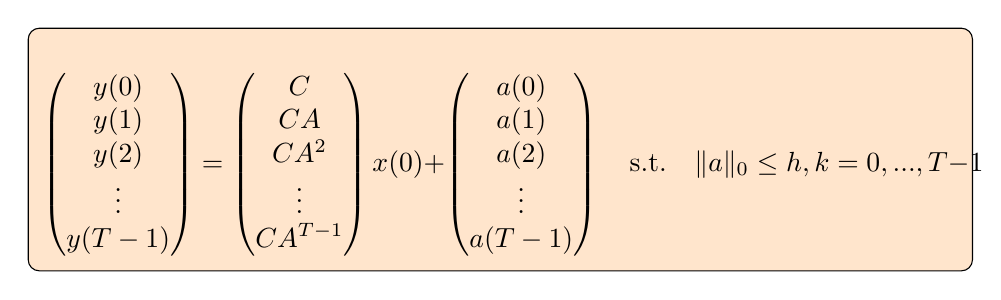
\begin{tikzpicture}
\node [mybox] (box){%
    \begin{minipage}{.96\textwidth}     %Larghezza del box
           \begin{equation*}
    \begin{pmatrix} y(0)\\ y(1)\\ y(2)\\   \vdots\\    y(T-1) \end{pmatrix} 
    =
    \begin{pmatrix}
        C\\ CA \\ CA^2 \\ \vdots \\ CA^{T-1} 
    \end{pmatrix} x(0) + 
     \begin{pmatrix} a(0)\\ a(1)\\ a(2)\\   \vdots\\    a(T-1) \end{pmatrix} 
     \quad \textrm{s.t.} \quad  \lVert a \rVert_0 \le h,  k=0,..., T-1
\end{equation*}
    \end{minipage}
};
\end{tikzpicture}%


\noindent
had a \textbf{unique solution}.



\noindent
Now we have to face with two problems: 
\begin{enumerate}  
    \setlength\itemsep{0em}
    \item Under \textbf{which conditions} can I solve the proposed problem?
    \item \textbf{How can I solve} it?
\end{enumerate}

\noindent
\section{Well-Position of the problem (Static case)}
Let us analyze the problem in a very particular case, that is when the system we want to ovbserve is \textbf{static}. That is the matrix $A\in \mathbb{R}^{n,n}$ is the identity matrix $\mathbb{I}_n$. This corresponds to state that $x(k+1)=x(k)=x$ (remember that we have no input $u(t)$).\\
In this case the observability matrix has a very simple form, in particular it is equal to the matrix $C\in\mathbb{R}^{q,n}$. We have that the problem becomes: 
{   \large{
    $$y=Cx+a \quad \textrm{s.t.} \quad \lVert a \rVert_{0} \le h$$ }
}

\noindent
It is useful to give these formal definitions:\\
\begin{lemma}[h-sparsity]
    A vector is said to be \textbf{h-sparse}, if  $\lVert a \rVert_0 = h  $
\end{lemma}

\begin{lemma}[Support]
    Given $a\in \mathbb{R}^q$ we denote with $Supp(a)=\{i: a_i \ne 0\}$, the set of i such that the i-th component of the vector is a non-zero number.
\end{lemma}

\noindent
{\color{red} \textbf{How the attack could be done in order to not to be 'detectable'?}}
 Let's consider an $a=Cw, \quad w \in \mathbb{R}^n, w \ne 0$ and assume it is that $\lVert Cw \rVert_0 \le h$ (for the assumption we made). We sobstitute in the equation and obtain:
$$y=Cx+Cw=C(x+w) \quad \textrm{s.t.} \quad \lVert Cw \rVert_0 \le h$$
Actually, if such $w$ exixts, the \textbf{attack is feasible} and so not detectable. This property depends strongly on the property of the matrix $C$.\\
Fortunately we have a \textbf{proposition} that provide us with an equivalence to determine the \textbf{resilience} of the system to h  attacks.


\vspace{0.3cm}

 \hspace*{0mm}
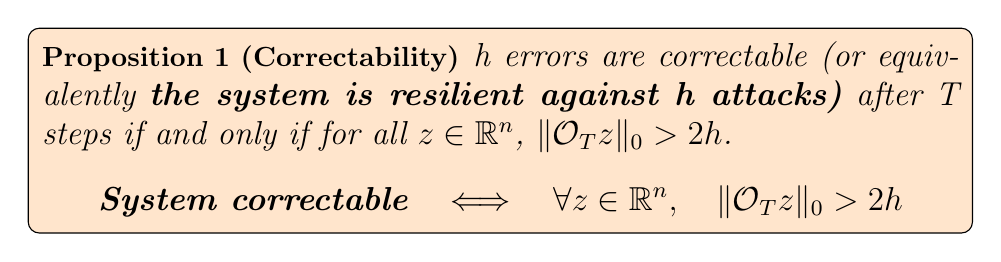
\begin{tikzpicture}
\node [mybox] (box){%
    \begin{minipage}{.96\textwidth}
          \begin{proposition}[Correctability]
    \large{
    h errors are correctable (or equivalently \textbf{the system is resilient against h attacks)} after T steps if and only if for all $z\in\mathbb{R}^n$, $\lVert \mathcal{O}_Tz \rVert_0 > 2h$.}
    $$\textrm{\textbf{System correctable}} \quad \Longleftrightarrow \quad \forall z \in \mathbb{R}^n , \quad \lVert \mathcal{O}_Tz \rVert_0>2h$$
\end{proposition}
    \end{minipage}
};
\end{tikzpicture}%

\noindent
In the static case the Proposition 1 becomes: $$\textrm{\textbf{System correctable}} \quad \Longleftrightarrow \quad \forall z \in \mathbb{R}^n , \quad \lVert Cz \rVert_0>2h$$
\begin{proof}
    As this is a characterization property we have to proof the proposition in the two direction $\Leftarrow$ and $\Rightarrow$. We give this proof for the static case, but the procedure for the more general case is analogue.
    \begin{itemize}
        \item {\Large{\textbf{[Proof of $\Leftarrow$] }}}
        {\color{blue} Assuming that 
        $\forall z \in \mathbb{R}^n$ we have $\lVert Cz \rVert_0 > 2h $ we want to demonstrate that h errors are correctable}, that is the problem has a unique solution.  As in many situation we want to demonstrate the uniqueness of something, we can go on \textbf{by contraddiction}. In particular assume that $y=Cx+a$ s.t. $\lVert a \rVert_0 \le h$ has got two different solutions: 
        $$\begin{pmatrix}
            x'\\ a'
        \end{pmatrix} and \begin{pmatrix}
            x''\\a''
        \end{pmatrix}$$

        then we have that $y=Cx'+a' \quad \textrm{s.t.} \quad \lVert a' \rVert_0 \le h$ but also $y=Cx''+a'' \quad s.t. \quad \lVert a'' \rVert_0 \le h $. $Cx'+a'=Cx''+a''$ $\Longleftrightarrow C(x'-x'')=a''-a'$ But due to the fact that $a'$ and $a''$ are h-sparse we can obtain by substracting them a vector which is \textbf{at most} 2h-sparse. 
        We have finished because we found a contradiction , that is, $\exists  z \in \mathbb{R}^n, \lVert Cz \rVert_0 \le 2h$. In this case $w=a'-a''$
        
        \item {\Large{\textbf{[Proof of $\Rightarrow$] }}}{\color{blue} Assuming that h errors are correctable,  we want to demonstrate that 
        $\forall z \in \mathbb{R}^n$ we have $\lVert Cz \rVert_0 > 2h $ }. Similarly the former case,  we can demonstrate the property by contradiction assuming that $\exists w \in \mathbb{R}^n \quad \lVert Cw \rVert_0 \le 2h$. We can write such $Cw$ like a sum of two (at most) h-sparse vectors $g_1$ and $g_2 \rightarrow Cw=g1+g2$. But we can also say that $Cw=g_1+g_2 \longleftrightarrow Cw-g_1=g_2=C 0+g_2 $. In this way we are saying that we have \textbf{two distinct solutions}, this is in contradiction with our hypotesis. \texttt{QED}
    \end{itemize}
\end{proof}

\noindent
The proposition that has just been proved is very powerful, but how are we able to try for all $z$ that the statement is valid? In the great majority of the situations is easier to provide a \textbf{counter-example}.\\
Now we are going to do some example and then to provide (at least) a necessary condition for well-position of the problem of correctability. 

\subsection{Some examples}
{\color{orange}\subsubsection{Example 0: a "naive" example}}
Consider that we have $C=\mathbb{I}_n$, $q=n$, $h=1$, $n=3$. In this case the output equation is: 
\begin{align*}
    &y_1=x_1\\
    &y_2=x_2\\
    &y_3=x_3
\end{align*}
As we can see the system is \textbf{perfectly observable} because each measurement of $y$ gives an element of the state, but suppose that we know that there is an attack ($h=1$), but we don't know where. If one of the measurement is corrupted, there is no way to recover the state of the system $\Rightarrow$ $C$ is not correcting h errors $\Rightarrow$ the system is not resilient to h attacks. In an intuitive way we can say that we could add more sensors to improve the situation, it is 'the path' that follows the next example.

{\color{orange}\subsubsection{Example 1: add more sensors (increase q)}}
At this point we change the (sensing) matrix $C$ by adding new measurements, so
$$C=\begin{pmatrix}
    1 &0 &0\\0& 1& 0\\0& 0 &1 \\ 1& 0& 0 \\ 0& 1& 0
\end{pmatrix}$$
What has changed here is that we have \textbf{two more }sensors. We have a duplication of $C_1$ and $C_2$ (we indicate with $C_i$ the i-th row of C). If $y_1=C_1x=y_4=C_4x$ and $y_2=C_2x=y_5=C_5x$ than we can state that the attack is on the sensor 3. But\textbf{ what if either $y_1 \ne y_4$ or $y_2 \ne y_5$}? We have no way to know which sensor has been attacked. If I switched off this couple of devices I can't observe anymore one of the component of the state vector. \\
This was only an \textbf{intuitive way} to understand this fact. How can we formalize it? 
We can say that the couple $(C_1, C_2)$ has a \textbf{non trivial kernel}. That is the equation:
$$\begin{pmatrix}
    1&0&0\\0&1&0
\end{pmatrix}z=\begin{pmatrix}
    0\\0
\end{pmatrix}$$
has a non zero solution. In particular a solution could be $z=\begin{pmatrix}
    0\\0\\\alpha
\end{pmatrix}$ such $z$ produces 
$$Cz=\begin{pmatrix}
    0\\0\\\alpha\\0\\0
\end{pmatrix} \quad \alpha \in \mathbb{R}$$ which due to the fact which is 1-sparse, is \textbf{in contradiction} with the proposition.\\
Conclusion: \textbf{even this matrix does not correct h=1 error $\Rightarrow$ the system \textbf{is not} resilient}!

{\color{orange}\subsubsection{Example 2: more mixed measurements}}
Freezing the other parameters, let us change again the matrix $C$ in the following way: 
$$C=\begin{pmatrix}
    1&0&0\\0&1&0\\0&0&1\\1&1&1\\1&-1&1
\end{pmatrix}$$
It is quite clear that there is a triple of rows of C which are linearly dependent, specifically $C_5=C_4-2C_2 \Rightarrow$ the triple has a non trivial kernel. By doing simple algebraic steps we desume that a solution could be  $z=\begin{pmatrix} 
    \alpha\\0\\-\alpha
\end{pmatrix}$ which generates a 2-sparse $Cz$ we have again a contradiction! Conclusion: \textbf{C is not resilient}. 

{\color{orange}\subsubsection{Example 3: linearly independent measurements}}
Now we provide the following $C$ matrix: 
$$C=\begin{pmatrix}
    &1&0&0\\&0&1&0\\&0&0&1\\&1&1&1\\&1&2&-1
\end{pmatrix}$$
In this case all the triples are linearly independent, this cause the relative kernel to be trivial $\rightarrow$ there is no way to produce a counter-example. 
Conclusion: this  $C$ matrix corrects h=1 error.

\subsection{A necessary condition for well-position}
Let $C\in \mathbb{R}^{q,n}$, $rank(C)=n$ and $q>n$, it is quite clear that any subset $\Omega$ composed by $n-1$ rows  has got a non trivial kernel. This implicates that the sparsity is not larger than $q-(n-1)$, that is $2h < q-(n-1)$ or equivalently $h \le q-n$. From which I can recover the following inequality: $$q\ge 2h+n$$
It is immediate to understand that if I want to correct $h=1$ error with $n=3$, we need at least of $q=5$ sensors.

This fact bring us to state that: 
\begin{itemize}
    \item Large $q$ is not sufficient for \textbf{resilience} 
    \item On the other hand there is a \textbf{minimum q} which I need to correct a certain number $h$ of errors.
\end{itemize}

\section{Reformulation of $y=Cx+a \quad \textrm{s.t.} \quad    \lVert a \rVert_0 \le h$}
\noindent
The second question to answer is: \\
{\begin{center}
\textbf{
    How can we solve the problem $y=Cx+a \quad \textrm{s.t.} \quad    \lVert a \rVert_0 \le h$?}
\end{center}} 
The problem can be reformulated as follows:
{   \large{
        $$\min_{x\in\mathbb{R}^n, a\in\mathbb{R}^q} \lVert a \rVert_0 \quad \textrm{s.t.} \quad y=Cx+a$$
    }
}\\
It can be proved that \textbf{if the system is resilient to h attacks the solution to this problem corrects h errors}. Unfortunately, even this form of the problem has its drawbacks: 
\begin{itemize}
    \item As the problem is a combinatorial one, is \textbf{not feasible} (NP-Hard)
    \item The \textbf{objective function} which contains an $\ell_0$ norm is \textbf{not convex, non continuous and non differentiable in 0}
\end{itemize}
The solution is going in the direction of \textbf{convex relaxation}: 
\begin{enumerate}
    \item In the objective function, we choose to relax $\lVert a \rVert_0$ with its \textbf{best CONVEX approximation} $\lVert a \rVert_1$; it is \textsc{Convex}, \textsc{Continuous} but \textsc{Non differentiable in 0} (we can face this problem);
    \item In the real world, we must take into account the noise that could appear in the equation $y=Cx+a$ and so it becomes $y\approx Cx+a$, this leads to the \textbf{Least Squares (LS) problem} $$\min{ \frac{1}{2}\lVert y-Cx-a \rVert_2^2}= 
    \min{\frac{1}{2}\Bigg\lVert y - \begin{pmatrix}
        C & I 
    \end{pmatrix}\begin{pmatrix}
        x\\
        a
    \end{pmatrix} \Bigg\rVert}$$ 
\end{enumerate}

Combining this two approximations, due to the fact we want to minimize both the terms, the \textbf{resulting problem to solve} is: 

\hspace*{-5mm}
\begin{center}
    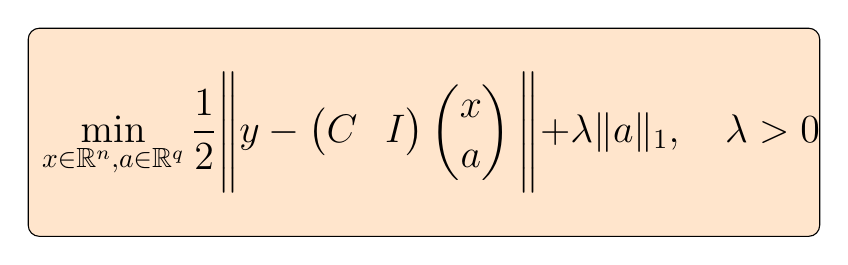
\begin{tikzpicture}
    \node [mybox] (box){%
        \begin{minipage}{.80\textwidth}
                %Qui testo
                {
                \color{black}
                \Large{
                    $$
                    \min_{x\in\mathbb{R}^n, a\in\mathbb{R}^q}{\frac{1}{2}\Bigg\lVert y - \begin{pmatrix}
                        C & I 
                    \end{pmatrix}\begin{pmatrix}
                        x\\
                        a
                    \end{pmatrix} \Bigg\rVert}+\lambda\lVert a \rVert_1, \quad \lambda>0
                    $$
                }}
                
        \end{minipage}
    };
    \end{tikzpicture}%
\end{center}



\subsection{Why $\ell_1$-regularization promotes sparsity?}
\begin{figure}[h]
    \centering
    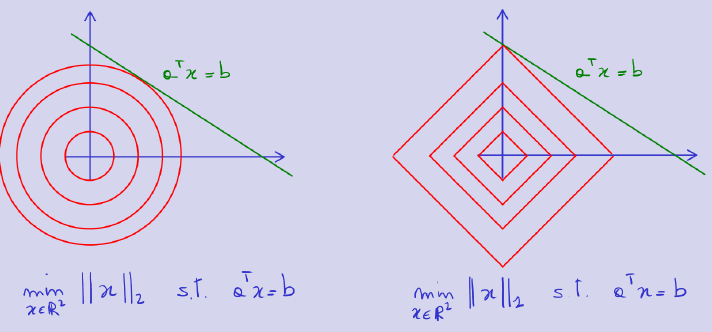
\includegraphics[scale=0.8]{images/Sparsity.png}
    \caption{$\ell_p$-norms and sparsification}
    \label{fig:enter-label}
\end{figure}
In the approximation we have just made, we have considered the $\ell_1$-norm. But why it is the best we could do? Let us consider to solve the problem $$\min_{x\in\mathbb{R}^2} \lVert x \rVert_2 \quad  \textrm{s.t.} \quad a^Tx=b$$ 
The term $\lVert x \rVert_2=k, k\in\mathbb{R}$ is a circle in the plane. We start from $k=0$, and we increase it until we reach the line to satisfy the (linear) constraint. The solution we obtain is certainly not sparse because it is of the form $x^*=(x_1^*, x_2^*)$ both non-zero real number.\\
\noindent
On the other hand if we consider the problem: 
$$\min_{x\in\mathbb{R}^2} \lVert x \rVert_1 \quad  \textrm{s.t.} \quad a^Tx=b$$ 
we note that the solution we can find (by using the same method as before) is sparse. We have seen in an intuitive way that $\ell_2$-norm takes the components of the solution close to zero in a "democratic way", in other words without 'reset' any component. At the opposite the $\ell_1$-norm push to zero \textbf{only some components} making a selection among them $\longleftrightarrow $ this promotes \textbf{"sparsification"}.\\

\noindent
{
    \color{blue}
    [Note that we have just showed a trivial way to understand why we have chose one regularization instead of another. The topic would require a more accurate and rigorous explanation, which we don't care.]
}

\subsection{Some observations}

\subsubsection{The problem has a connection with LASSO}
The problem we found to solve after applying \textbf{relaxation} is very similar to the problem of \textbf{LASSO} (Least Absolute Shrinking and Selection Operator) in fact in its original formulation we have: 
$$\min_{x\in\mathbb{R}^n} \frac{1}{2}\lVert Ax-y \rVert_2^2+\lambda\lVert x \rVert_1$$
but this give an entire sparse solution. In our problem only a piece of the solution is sparse, whose linked to attacks $a$, so we can see our problem as a "\textbf{Partial LASSO}" because we have \textbf{no regularization} on the term $x$ of the solution $\begin{pmatrix}
    x\\a
\end{pmatrix}$.

\subsubsection{The problem has a connection with "Compressed Sensing"}
The problem
 $$
    \min_{x\in\mathbb{R}^n, a\in\mathbb{R}^q}{\frac{1}{2}\Bigg\lVert y - G\begin{pmatrix}
        x\\
        a
    \end{pmatrix} \Bigg\rVert}+\lambda\lVert a \rVert_1, \quad \lambda>0,
    \quad 
    G=\begin{pmatrix}
        C & I 
    \end{pmatrix}
    $$
as the $G$ matrix has more columns than rows, is a \textbf{fat matrix} and without regularization the problem has infinitely many solutions. We can consider the $y$ a \textbf{linear compressed measurement} vector.
The problem of \textbf{recover a sparse vector from compressed linear measurement} has a strong connection with the \textsc{Compressed sensing} problem. Also here we have a \textbf{"Partial Compressed Sensing"} as only a part of the solution is sparse.\\

\noindent
{
\large{
    \color{red}
    After a "long journey" we have understood that for the \textbf{secure state estimation of CPS under adversarial attacks} we have to solve a \textbf{Partial LASSO} problem. For this reason we seek a way to solve it $\Rightarrow$ Iterative Algorithms
    }
}
    
\section{IST: an algorithm for LASSO}
\noindent
{\color{blue}
\textit{
    \textbf{Premise} In this course we will not see any black box technique, we will go through the direction of \textbf{iterative algorithms} to solve the LASSO problem.\\
    \noindent
    In the framework of \textbf{Convex Optimization} one of the most used algorithms (also in Data Science/Machine Learning...) is the \textbf{Gradient Descent Algorithm}. But in the LASSO we have a $\ell_1$-regularization, which is not differentiable in 0. We can't even avoid to consider it because we want to reach the (global) \textbf{minima}. We wonder if using an approximation could be the solution (eg. \textbf{subgradients}), however again this not produce a \textit{sparse solution}. 
}\\
}

\noindent
Once the proper promises have been done, we can introduce this algorithm for solving the \textbf{(sparse) optimization problem} of LASSO. 
The algorithm is called \textbf{Iterative Shrinkage/Thresholding (IST)} and it is a variant of the \textit{Descent Gradient Algorithm}. After the definition and a general description, we are goingo to list the steps of the algorithm itself. Initially we consider the original LASSO problem
$$\min_{x\in\mathbb{R}^n} \frac{1}{2}\lVert Ax-y \rVert_2^2+\lambda\lVert x \rVert_1$$ in which we call $F(x)=\lVert Ax-y \rVert_2^2$ the Least-Squares functional. Moreover we know that $\nabla F(x) = A^T(Ax-y)$.\\

\noindent
\textbf{Definition (Shrinkage/Thresholding operator)} The \textbf{Shrinkage/Thresholding operator} $\mathbb{S}_{\alpha}$ is a component wise operator $\mathbb{S}_{\alpha}: \mathbb{R}^p \rightarrow \mathbb{R}^p, \alpha >0$. For any $x_i\in \mathbb{R}$:
\begin{equation*}
    \mathbb{S}_{\alpha}(x_i) =
        \begin{cases}
            x_i-\alpha & \text{if $x_i$>$\alpha$} \\
            x_i+\alpha & \text{if $x_i$ < -$\alpha$}\\
            0 & \text{if $ \lvert x_i \rvert \le \alpha$}\\ 
        \end{cases}
\end{equation*}



\hspace*{-5mm}
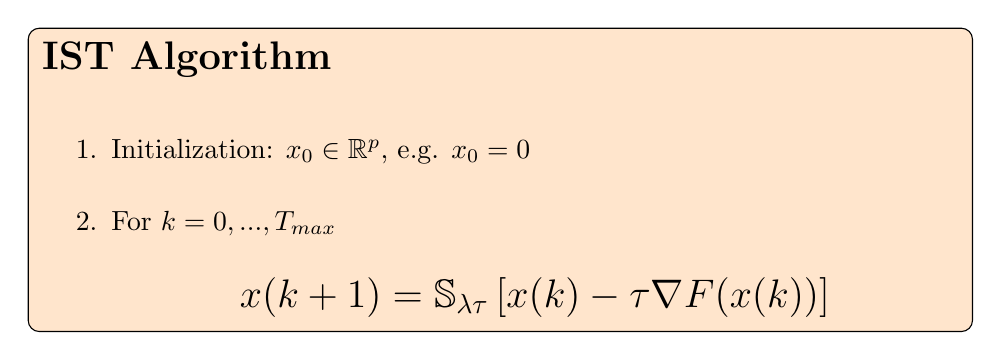
\begin{tikzpicture}
\node [mybox] (box){%
    \begin{minipage}{.96\textwidth}

    \textbf{\Large{IST Algorithm}}\\
        \begin{enumerate}
            \item Initialization: $x_0\in\mathbb{R}^p$, e.g. $x_0=0$
            \item For $k=0,..., T_{max}$
            \Large{
            \begin{equation*}
                x(k+1)=\mathbb{S}_{\lambda \tau} \left[ x(k)-\tau\nabla F(x(k))
                \right]
            \end{equation*}
            }
        \end{enumerate}
    \end{minipage}
};
\end{tikzpicture}%

\vspace{0.5cm}
\noindent
The parameter $\tau$ has to be "small enough" so that the algorithm works as desidered. It has been demonstrated that the algorithm converge to the minimum of the LASSO functional $\frac{1}{2}\lVert Ax-y \rVert_2^2+\lambda\lVert x \rVert_1$. The \textbf{iterative nature} and simplicity of this method, makes it adaptable also for: \textbf{dynamic} and \textbf{distributed} systems.

\subsection{Derivation of IST Algorithm} 
Let us do a quick RECAP of the latest notions we introduced...\\
Generally speaking, when we have some measurements $y=A\tilde{x}+\eta$ where $\tilde{x}$ is the \textbf{true vector} to recover, we are able to find an \textbf{estimate} of it by solving the problem 
$$x^{*} = \textrm{arg} \min_{x\in \mathbb{R}^n} \frac{1}{2}\lVert y-Ax \rVert_{2}^{2}$$
also known as the \textbf{Least Squares (LS)} problem, where the obtained $x^*$ is the estimate of the true vector. How can we solve this problem?\\
The \textbf{Gradient Descent} method is one of the most used in this field to retrieve a solution for LS problem. This algorithm step by step proceeds in the direction of the gradient, moving from the previous point of a \textbf{step size} called $\tau$ (small enough). Then we have 
\begin{equation} 
\label{eq:1}
    x(k+1)=x(k)-\tau \nabla{F(x)}, \quad F(x)= \lVert y-Ax \rVert_2^{2} \quad \textrm{(LS functional)}
\end{equation}
 for $k=0,1, 2, ....$  \\
We can observe that the expression (\ref{eq:1}) is a Discrete Time Linear Time Invariant System (DT LTI), therefore we can study its properties by using the known results from the Theory.\\

Differently from the case which has just mentioned, in the LASSO problem we have the {$\ell_1$-norm} too, because we are interested in finding a \textbf{sparse solution} (in our framework of \textbf{CPS under adversarial attacks} this is an important requirement). It is good to remind that the LASSO is a \textbf{convex, non-differentiable} problem. \\
Then, how can we solve it? Its solution can be retrieved by using any convex optimization solver (\texttt{cvx,lasso, ...}). On the other hand, the \textit{Gradient Descent} algorithm is not effective! (Gradient of a non differentiable functional?? We can't!). Our \textbf{approach} is using the \textbf{ISTA} Algorithm of which it is given a \textbf{possible interpretation}. \\

Let the functional $F(x)=\frac{1}{2}\lVert y-Ax \rVert_{2}^{2}+\lambda\lVert x \rVert_1$ be the LASSO functional. We define now a \textbf{surrogate functional} which will guide our \textit{derivation of ISTA} as 
\begin{equation}    \label{eq:SurrogateFunctional}
    \mathcal{R}(x,b)=F(x)+\frac{1}{2\tau}\lVert x-b \rVert_2^2 -\frac{1}{2} \lVert Ax-Ab \rVert_2^2,
    \quad \tau > 0
\end{equation}
where $x$ is my 'standard' variable, while $b$ is an auxiliary variable. By using a little bit of linear algebra we note that:  
\begin{align*}
    &\frac{1}{2\tau}\lVert x-b \rVert_2^2 -\frac{1}{2} \lVert Ax-Ab \rVert_2^2 =
    \frac{1}{2\tau}\lVert x-b \rVert_2^2-\frac{1}{2} \lVert A \rVert_2^2 \lVert x-b \rVert_2^2=
    \frac{1}{2}  \bigg( \frac{1}{\tau} - \lVert A \rVert_2^2 \bigg) \lVert x-b \rVert_2^2
\end{align*}
and this quantity is non-negative if and only if $\frac{1}{\tau} > \lVert A \rVert_2^2 \Rightarrow \tau < \lVert A \rVert_2^{-2}$. This provides a guide to choose the $\tau$  and ensures that the \textbf{surrogate part} of the functional (\ref{eq:SurrogateFunctional}) is never negative, moreover it can immediately be noted that it is null if and only if $x=b \Rightarrow F(x)=R(x,x)$. That is the global minimum of $F(x)$ is the same of the global minimum of $R(x, x) \Rightarrow F(x^*)=R(x^*, x^*)$. At this point: our aim is to develop a \textbf{descent algorithm} for $F(x)$ which we will see that it is eased by $R(x, b)$.\\

It is not trivial to find a closed form for the solution of minimizing the surrogate functional considering both variables $x, b$ together. Therefore, we move in the direction of an \textbf{alternating minimization} (alternating $\Rightarrow$ in turn). This is both \textbf{feasible} and \textbf{leads to the minimum} of $F(x)$. More clearly:

$$\begin{cases}
    \min_{b\in \mathbb{R}^n } \mathcal{R}(x,b),& \quad \text{keeping $x$ as a constant} \\
    \min_{x \in \mathbb{R}^n} \mathcal{R}(x,b),&  \quad \text{keeping $b$ as a constant}
\end{cases}$$

\subsubsection{First step: minimizing with respect to $b$}
It is more trivial because we have seen recently that the \textit{surrogate part} depends on b, and it is minimum if $x=b$, then   
$$x=\textrm{arg}\min_{b \in \mathbb{R}^n} \mathcal{R}(x,b) $$

\subsubsection{Second step: minimizing with respect to $x$}
The problem here is find $\textrm{arg}\min_{x \in \mathbb{R}^n} \mathcal{R}(x,b)$. In this case we have to expand the functional by expressing the squared norm explicitly, to reach a conclusion. 
\begin{align}
\textrm{arg}\min_{x \in \mathbb{R}^n} \quad 
    &\mathcal{R}(x,b)=
    \textrm{arg}\min_{x \in \mathbb{R}^n} \quad 
    \frac{1}{2} \lVert Ax \rVert_2^2 +\frac{1}{2} \lVert y \rVert_2^2-yA^Tx+\lambda\lVert x \rVert_1+\\
    & \frac{1}{2\tau} \lVert x \rVert_2^2 + \frac{1}{2\tau} \lVert b \rVert_2^2-\frac{1}{\tau}b^Tx+\\
    &-\frac{1}{2}\lVert Ax \rVert_2^2 - \frac{1}{2}\lVert Ax \rVert_2^2 -b^TA^TAx = \\
    \label{eq: expanded}
    \textrm{arg}\min_{x \in \mathbb{R}^n} \quad 
    &\lambda \lVert x \rVert_1+\frac{1}{2\tau}\lVert x \rVert_2^2-x^T 
    \bigg( \frac{1}{\tau}b+A^Ty-A^TAb \bigg) =\\
    \label{eq:mult_tau}
    &\tau \lambda \lVert x \rVert_1 + \frac{1}{2} \lVert x \rVert_2^2 - x^T [b+\tau A^T(y-Ab)]+\frac{1}{2}\lVert b+\tau A^T(y-Ab) \rVert_2^2=\\
    \label{eq:final_step}
    \textrm{arg}\min_{x \in \mathbb{R}^n} \quad 
    &\tau\lambda\lVert x \rVert_1 + \frac{1}{2} \lVert x-q \rVert_2^2=
     \textrm{arg}\min_{x \in \mathbb{R}^n} \quad 
    \sum_{i=1}^{n} \bigg(\tau\lambda \lvert x_i \rvert + \frac{1}{2} (x_i-q_i)^2 \bigg)
\end{align}

In (\ref{eq:mult_tau}), by multiplying all terms in (\ref{eq: expanded}) by $\tau$ and by adding a constant term ${q= b+\tau A^T(y-Ab)}$ nothing change. Moreover the final step (\ref{eq:final_step}) is separable, in the sense that If I want minimize the sum, I can proceed \textbf{component wise}. Therefore

\begin{align}
     \textrm{arg}\min_{x \in \mathbb{R}^n} \quad 
    \sum_{i=1}^{n} \bigg(\tau\lambda \lvert x_i \rvert + \frac{1}{2} (x_i-q_i)^2 \bigg)
    &\Longleftrightarrow
     \textrm{arg}\min_{x_i \in \mathbb{R}} \quad
    \tau\lambda \lvert x_i \rvert + \frac{1}{2} (x_i-q_i)^2 = (...)=
\end{align}

\begin{equation}
    =\begin{cases}
        q_i-\tau\lambda &\quad \text{if}\quad q_i>\tau\lambda\\
        q_i+\tau\lambda\ &\quad \text{if}\quad q_i<-\tau\lambda\\
        0 &\quad \text{if}\quad q_i\in[-\tau\lambda, \tau\lambda]\\
    \end{cases}
\end{equation}
but this is the operator we formerly introduced as $\mathbb{S}_{\tau\lambda}(q)$ which pushes the component of the vector $q$ close to zero. We can reach a \textbf{conclusion}.\\
\noindent
Given $x_0=0$ for any $k=0,1,...$
\begin{enumerate}
    \item $b(k+1) =    \text{arg}\min_{b\in\mathbb{R}^n} \mathcal{R}(x(k),b)=x(k)$
    \item $x(k+1)=\text{arg}\min_{x\in\mathbb{R}^n} \mathcal{R}(x,b(k+1))=
    \text{arg}\min_{x\in\mathbb{R}^n} \mathcal{R}(x,x(k))=
    {\mathbb{S}_{\tau\lambda}[x(k)+\tau A^T(y-Ax(k))]}$
\end{enumerate}
Then, 
\begin{equation}\label{eq:ISTA_eq}
    x(k+1)={\mathbb{S}_{\tau\lambda}[x(k)+\tau A^T(y-Ax(k))]}
\end{equation}
which is our \textbf{Iterative Shrinkage/Thresholding algorithm (ISTA)}. Then, at the end of this discussion we have seen that the algorithm on which we focus comes from an \textbf{alternating minimization} of the surrogate functional $\mathcal{R}(x, b)$.\\

\hspace*{-5mm}
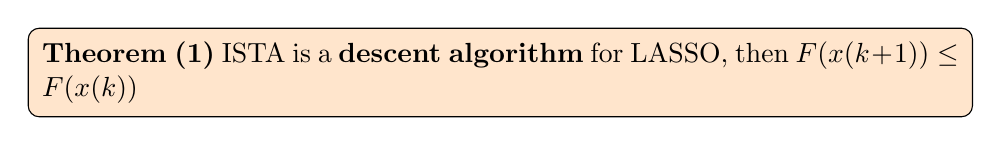
\begin{tikzpicture}
\node [mybox] (box){%
    \begin{minipage}{.96\textwidth}     %Larghezza del box
           \textbf{Theorem (1)} ISTA is a \textbf{descent algorithm} for LASSO, then $F(x(k+1))\le F(x(k))$
    \end{minipage}
};
\end{tikzpicture}

\textbf{Proof} The proof of the theorem above is very simple:
\begin{align*}
    F(x(k))=&\mathcal{R}(x(k), x(k))  \ge \quad &\text{(minimizing over x)} \\
    &\mathcal{R}(x(k+1), x(k))  \ge \quad &\text{(minimizing over b)}\\
    &\mathcal{R}(x(k+1), x(k+1)) = F(x(k+1),x(k+1))
\end{align*}

\hspace*{-5mm}
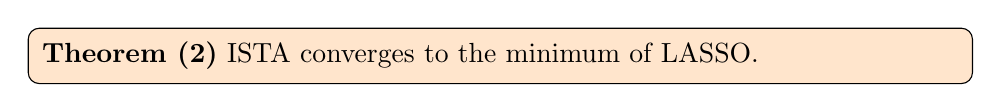
\begin{tikzpicture}
\node [mybox] (box){%
    \begin{minipage}{.96\textwidth}     %Larghezza del box
           \textbf{Theorem (2)} ISTA converges to the minimum of LASSO.
    \end{minipage}
};
\end{tikzpicture}

\subsection{Curiosity}
The equation (\ref{eq:ISTA_eq}) combines a linear part (the argument of the operator $\mathbb{S}$) and a \textbf{non linear part} that is the operator itself, being defined in a piece-wise fashion. The resulting system is a \textbf{Discrete Time Non Linear Time Invariant system} which is not trivial to treat.\\
This reminds a little the structure of a \textbf{neural network} where we have a \textbf{linear part} and a \textbf{non linear part} constituted by the \textbf{activating function}. For this reason the \textbf{evolution of ISTA} can be seen as a \textbf{Neural Network} application.

\subsection{Application of ISTA on CPS framework} 
We have seen recently that the problem of Cyber-Physical system under attacks can be formulated as follows: 
\begin{equation}
    \min_{x \in \mathbb{R}^n, a \in \mathbb{R}^q} 
    {\frac{1}{2} \bigg\lVert y-G \begin{pmatrix}
        x\\a
    \end{pmatrix} \bigg\rVert + \lambda \lVert a \rVert_1}
\end{equation}
that is a \textbf{partial LASSO} because only a part of the found solution is sparse, whose related to the (sparse) attacks. What about ISTA for Partial LASSO?
I have no limitations about the choice of the coefficient $\lambda$, in particular I can get $\lambda=0$ for the elements of the solution which are not interested by sparsity as it is the state of the system. Then, 
\begin{equation}
    \lambda\lVert a \rVert_1 = \lambda\bigg\lVert \begin{pmatrix}
        x\\a
    \end{pmatrix} \bigg\rVert_1 = 0\lvert x_1 \rvert+...+0\lvert x_n \rvert+
    \lambda \lvert a_1 \rvert + \lambda \lvert a_q \rvert
\end{equation}
This changes nothing, but it is essential that we made this variation in a way that the derivated descent algorithm could fit the "Partial LASSO" problem used for CPS purposes.


\chapter{Localization by RSS fingerprinting}
\section{Introduction}
\noindent
\textbf{Localization} is the problem related to the \textbf{estimation} of the position of a \textbf{target}. Other problems are those related to the \textbf{detection} (whether a target is present or not) and \textbf{tracking} that is we track the position of a \textbf{moving target}.\\
Nowadays the focus is in particular on \textbf{Indoor Localization} whose mathematical modeling is quite challenging due to the presence of \textit{multipath} and \textit{reflecting surfaces}. For these reasons there is not an available \textbf{unified approach}. \\
GPS is not usable for indoor localization, the so called \textbf{WSN (Wirelless Sensor Networks)} are used for this purpose. A WSN is essentially a network of devices equipped  with sensors. We can find two main approaches: 
\begin{enumerate}
    \item \textbf{Triangulation and Trilateration}: in this case we assume that the target is a \textbf{transmitting device} that broadcasts a signal. The former method deploy the \textbf{direction of arrival} of such signal, the latter use instead the \textbf{distance} from the source's signal (\textit{id est} the target). For this approach, in the case that the measurement are exact, 3 non-aligned sensors are sufficient, alternatively the higher number of sensors, the higher precision reached.
    \item \textbf{Fingerprinting methods} refers to techniques that match the \textbf{fingerprint} of some characteristics of a signal which is \textbf{location-dependent}. For our purposes we consider the \textbf{Received Signal Strength} or \textbf{RSS}.
\end{enumerate}

\section{RSS-fingerprinting: general description }
In general for all \textbf{Fingerprinting method}, we identify \textbf{two phases}:
\begin{enumerate}
    \item \textbf{Training phase} in which we collect the fingerprints of a scene; 
    \item \textbf{Runtime phase} in which we match the online measurement with the closest a-priori location fingerprints.
\end{enumerate}
As we said, we focus our attention on \textit{RSS-fingerprinting}.

\subsection{(Phase 0) Initialization }
Given the room where the localization has to be done, we deploy the WSN in some way (For example: grid deployment, or random (uniform) deployment, split the room into $p$ cells.   \textbf{Localize the target} $\longrightarrow$ detect in which cell the target is placed.

\begin{figure}[h]
    \centering
    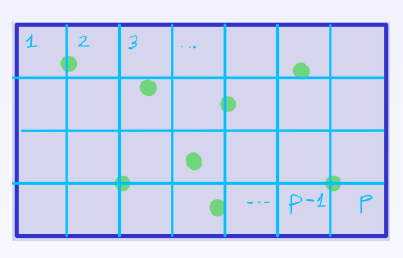
\includegraphics{images/RSS-cells.png}
    \caption{(Phase 0) - Initialization}
    \label{fig:RSS-Cells}
\end{figure}

\subsection{(Phase 1) Training phase}
We put the target in each cell. According to the fact that the target itself broadcasts a signal, \textbf{each sensor} measures and stores the RSS, and create a \textbf{signature map} or \textbf{dictionary}. More specifically, the dictionary can be represented by a matrix $D$, in which each entry $D_{i,j} $ denotes the RSS-measurement the sensor $i$ takes when the target is in the $j$-th cell. \\
\textbf{Each sensor} builds its own dictionary, and the WSN builds an \textbf{overall dictionary} $D\in \mathbb{R}^{q,p}$.\\
This phase takes some time and requires that the nodes of the network saved the information, it makes the runtime phase more accurate. 

\begin{figure}[h]
    \centering
    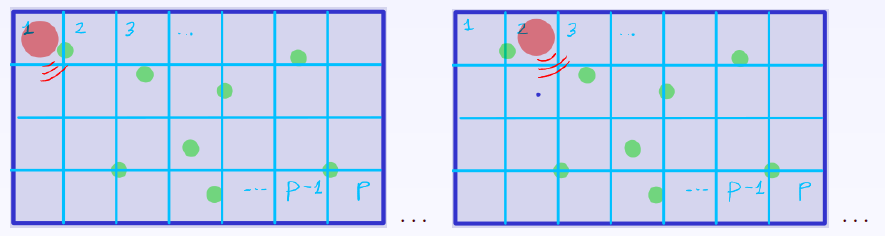
\includegraphics[scale=0.8]{images/RSS-training.png}
    \caption{(Phase 1) - Training phase}
    \label{fig:enter-label}
\end{figure}

\subsection{(Phase 2): Runtime phase}
Is the phase in which the localization is performed. Each sensor takes a measurement $y_i$, the $j$-th column of the dictionary indicates the $j$-th cell of the room in which the target is located!  

\begin{figure}[h]
    \centering
    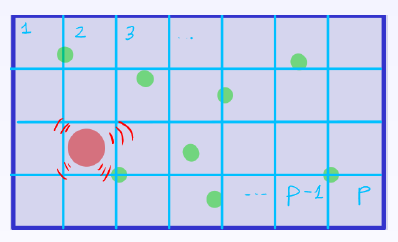
\includegraphics{images/RSS-Runtime.png}
    \caption{(Phase 2) - Runtime phase}
    \label{fig:enter-label}
\end{figure}

\noindent
If there is one target, then one of the columns of the dictionary would correspond to the measurement (in theory), then the target is located in the $j$-th cell where $j$ is such that $y=D_j$, with $D_j$ the $j-th$ column of the dictionary but usually, we can have \textit{multiple target} in the same room moreover it's very difficult that $y=D_j$ due to the presence of noise on sensors.\\

Then, in this scenario we have that the vector of measurements $y$ is a sum of a subset of the columns of the matrix $D$, to which we must add an additional term related to the noise. We have: 
\begin{equation} \label{eq: prob_loc}
	y=Dx+\text{noise}
\end{equation}
Where $x\in\{0,1\}^p$ and $x_i=1$ when in the i-th cell there is a target. \\
A further observation which can be done is that, in the real problems of \textit{indoor localization} the number of the targets one would like to localize is \textbf{much smaller} than the number of the cells, this leads to the sparsity of the solution $x\in\mathbb\{0,1\}^p$. 
Summarizing: (i) We want to find a solution to the problem (\ref{eq: prob_loc}), (ii) We know that such solution is \textbf{sparse}. Then,
\begin{equation}
	x^*=\text{arg}\min_{x\in\{0,1\}^p} \frac{1}{2} \lVert y-Dx \rVert_2^2 + \lambda \lVert x \rVert_1
 \end{equation}
This type of formulation leads to a \textbf{mixed integer} combinatorial problem, that again is NP-hard, so non-tractable. We can relax the constraint $x\in\{0,1\}^p$ into $x\in\mathbb{R}^p$, obtaining:
\begin{equation} \label{eq: loc_LASSO}
	x^*=\text{arg}\min_{x\in\mathbb{R}^p} \frac{1}{2} \lVert y-Dx \rVert_2^2 + \lambda \lVert x \rVert_1
\end{equation}
This is the problem of LASSO in the original formulation. {\color{red} It is important to remember that: } the solution of the problem (\ref{eq: loc_LASSO}) is not the original $x$ due to: (i) the presence of the noise, (ii) a bias introduced by the $\ell_1$-regularization term which in part promotes sparsity on the other hand inserts an error. One can use of course the \textbf{IST Algorithm} to find a solution.

\section{Localization under sparse sensor attacks}
\noindent
Assume that, in a realistic way, the training phase is \textit{attack-free}, therefore the matrix $D$ is attack free. Let us focus the attention again in the runtime phase.\\
What if the sensors were under adversarial attacks? One can apply the theory we developed in the former chapter! Then, we assume that the sensors under attacks are much smaller than the total number $q$ of them. In this context the equation (\ref{eq: prob_loc}) becomes: 
\begin{equation}
	y=Dx+a+noise	
\end{equation}
Then, the formulation of problem changes as follows:\\


\hspace*{-5mm}
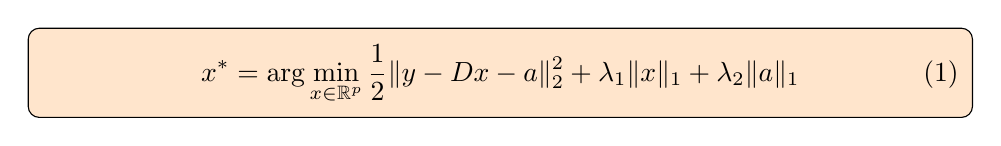
\begin{tikzpicture}
	\node [mybox] (box){%
		\begin{minipage}{.96\textwidth}     %Larghezza del box
			\begin{equation}
				x^*=\text{arg}\min_{x\in\mathbb{R}^p} \frac{1}{2} \lVert y-Dx-a \rVert_2^2 + 
				\lambda_1 \lVert x \rVert_1+
				\lambda_2\lVert a \rVert_1
			\end{equation}
		\end{minipage}
	};
\end{tikzpicture}


where we are using different weights $\lambda_1, \lambda_2$ to give more or less importance to the term related to the solution $x$ and to the attack $a$. According to this novel aspect, the risen problem is a \textbf{weighted LASSO}. \textbf{IST algorithm} continues to work, as we saw in the case of presence of \textit{non-sparse} part of the solution in the case of SSE under adversarial attacks.

\noindent
\section{Other approaches to Localization}
The approach we have just seen is not the only one. Next paragraphs are in order to give some alternatives which differ from the first we have presented in computational complexity, time of convergence and so on.

\subsection{k-Nearest Neighbour (K-NN)}
Assume to know that there is only \textbf{one target}, given the vector $y\in \mathbb{R}^q$, we could find the $j-th$ column of the dictionary $D$ that is the \textbf{nearest} with respect to $y$. The localization problem in this specific scenario becomes: 
\begin{equation} \label{eq:knn_1}
	\hat{j} = \text{arg}\min_{j=1,...,p} \lVert D_j-y \rVert_2^2
\end{equation}
where $D_j$  is the $j$-th column of $D$. Note that in the problem there is not the factor $\frac{1}{2}$ but from the moment we have a minimization problem nothing changes.\\
RSS is additive so we can localize more than one target in the \textit{runtime phase}. Suppose that the targets are $k=2$, the vector $y$ can be seen as a sum of the columns, so the problem (\ref{eq:knn_1}) gets transformed in:
\begin{equation}
	(\hat{j_1}, \hat{j_2}) = \text{arg}\min_{(j_1, j_2)=1,...,p} 
	\lVert D_{j_1}+D_{j_2}-y \rVert_2^2
\end{equation} 

In general, we have to check a number of configurations that is equal to $\binom{p}{k} \rightarrow$ \textbf{NP-Hard}. Note that: this approach can be used if we have small $p, k$ otherwise other techniques ought to be used in order to promote efficiency.

\subsection{Linear Regression (noise-free case)}
If we have multiple targets, in absence of noise the localization problem could be formulated as a \textbf{binary linear regression}. We have to solve in $x$ the equation $y=Dx$ and add the constraints about the $x$ domain and sparsity. Then, it is obtained:
\begin{equation}
	\begin{aligned}
		Dx&=y\\
		&\text{s.t.} \ x\in\{0,1\}^p, \ \sum_{j=1}^{p}x_j=k
	\end{aligned}
\end{equation}
Even in this case it has been risen a mixed-integer combinatorial problem $\rightarrow$ NP-Hard. The choice should be taken in an accurate way according to the dimension of the problem.

\section{Some comments on the setting}
These algorithms assume that there is a \textbf{Fusion Center} where data from the sensors are collected. In this way: the Fusion Center stores the whole dictionary $D$ and the runtime measurements, so that it can run the localization algorithm which is nothing but one of the exposed methods.


\chapter {Dynamic Secure State Estimation of CPSs under adversarial attacks}
It has been explained in the previous chapter that for a system 
\begin{equation} \label{eq:system}
	\begin{aligned}
		&x(k+1)=Ax(k)\\
		&y(k)=Cx(k)
	\end{aligned}
\end{equation}
if one collects $n$ measurements $y(i), i=1,..., n$, we can recover the state $x(k)$ at each $k$, if we are able to find $x(0)$ and then invert the equation
\begin{equation*}
	y = \mathcal{O}_n x(0)
\end{equation*}
the Theorem by Kalman, states that this is possible, that is the system is \textbf{observable}, if and only if $\text{rank}(\mathcal{O}_n)=n$.
This is the static-batch approach to the \textbf{state estimation problem}, on the other hand - as an alternative technique - if the system is observable we can estimate $x(k)$(then $x(0)$) dynamically by constructing a device called the \textbf{Observer}, in the deterministic case it is called \textbf{Luemberger Observer}.\\

\section{Review of Luemberger Observer}

A copy of the system (\ref{eq:system}) is made with the only difference of adding a correction term. Starting from this point we use $\hat{x}(k)$ to indicate the \textbf{estimate of the state at the time $k$} (discretized time), and $\hat{y}(k)$ is the output computed by using the estimate. The Luemberger Observer has the following equations: 
\begin{equation} \label{eq: Luemberger}
	\begin{aligned}
			&\hat{x}(k+1)=A\hat{x}(k)-L[\hat{y}(k)-y(k)]\\
		&\hat{y}(k)=C\hat{x}(k)
	\end{aligned}
\end{equation}
The quantity $e(k)=\hat{x}(k)-x(k)$ is the error of the estimate at time $k$, the aim is to design an online algorithm which could make $e(k)\rightarrow 0 $. \\
In order to understand the role of the matrix $L\in \mathbb{R}^{n,q}$,  called the \textbf{observer gain matrix}, we can write: 
\begin{align}
	e(k+1)&=\hat{x}(k)-x(k)=A\hat{x}(k)-L[\hat{y}(k)-y(k)]-Ax(k)=\\
	&=A\hat{x}(k)-LC\hat{x}(k)-LCx(k)-Ax(k)=\\
	&=A[\hat{x}(k)-x(k)]-LC[\hat{x}(k)-x(k)]=\\
	&=(A-LC) [\hat{x}(k)-x(k)]=\\
	&=(A-LC) \ e(k)	
\end{align}
The resulting equation $e(k+1)=(A-LC)\ e(k)$ describes an LTI discrete time dynamical system in which the state matrix is represented by $A-LC$. From the theory of dynamical systems, we know that the system is asymptotically (internally) stable if after a certain time $k$, it is verified that $e(k)\rightarrow 0$, the result we are seeking, it is verified when the \textit{eigenvalues} of $A-LC$ are in the unitary circle. \\

Regarding the matrix $A$ it is not very interesting to track $x(k)$ if it is asymptotically stable because in this situation $\lim_{k \to \infty} x(k)=0$. So $A$ is required to be stable but not asymptotically (some authors refers to this type of stability as \textbf{marginal stability}).\\

\hspace*{-5mm}
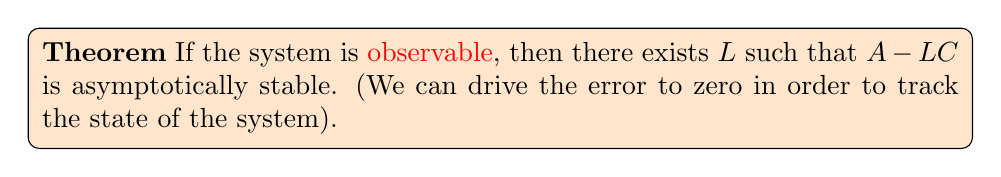
\begin{tikzpicture}
	\node [mybox] (box){%
		\begin{minipage}{.96\textwidth}     %Larghezza del box
			\textbf{Theorem} If the system is {\color{red}observable}, then there exists $L$ such that $A-LC$ is asymptotically stable. (We can drive the error to zero in order to track the state of the system).
		\end{minipage}
	};
\end{tikzpicture}

\section{State estimation by Least-squares approach}
At a certain time $k$, given the current measurement $y(k)=Cx(k)$, we might estimate $x(k)$ by solving the following problem: 
\begin{equation}
	\hat{x}(k) = \text{arg}\min_{x\in\mathbb{R}^n} \frac{1}{2} 
	\lVert y(k)-Cx \rVert_2^2 
\end{equation}
if $q>n$ and $C$ is full rank. We call $\mathcal{F}(x) =\frac{1}{2} 
\lVert y(k)-Cx \rVert_2^2$ the Least-Squares functional. 
There is a problem: the (pseudo)inversion of the matrix $C$, could be non-trivial for a medium-large dimensional problem. Even the classical Gradient Descent Algorithm would be too slow!\\
A solution is: at each $k$, we run a \textbf{single step} of gradient descent resulting in an \textbf{Online gradient descent}.\\

\hspace*{-5mm}
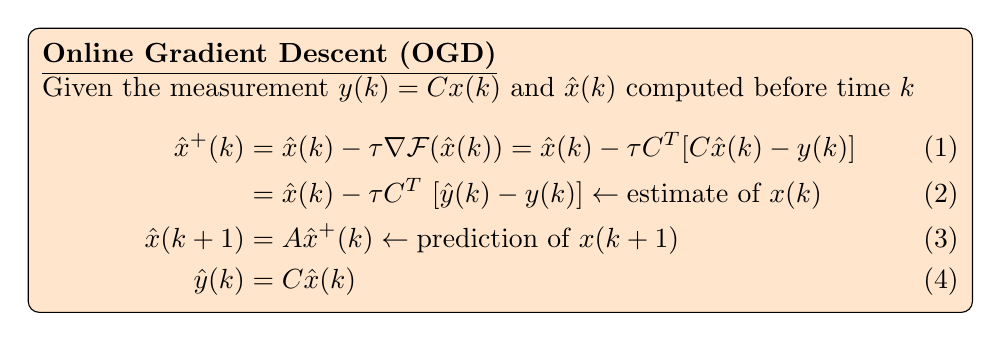
\begin{tikzpicture}
	\node [mybox] (box){%
		\begin{minipage}{.96\textwidth}     %Larghezza del box
				\textbf{\underline{Online Gradient Descent (OGD)}} \\
				Given the measurement $y(k)=Cx(k)$ and $\hat{x}(k)$ computed before time $k$
				\begin{align}
					\hat{x}^+(k)&=\hat{x}(k)-\tau\nabla\mathcal{F}(\hat{x}(k)) =  \hat{x}(k)-\tau C^T[C\hat{x}(k)-y(k)]\\
					&=\hat{x}(k)-\tau C^T  \ [\hat{y}(k)-y(k)] 
					\leftarrow \text{estimate of} \ x(k)\\
					\hat{x}(k+1)&=A\hat{x}^+(k) 
					\leftarrow \text{prediction of} \ x(k+1)\\
					\hat{y}(k)&=C\hat{x}(k)				
				\end{align}
		\end{minipage}
	};
\end{tikzpicture}
By merging estimate and prediction we obtain:
\begin{equation}\label{eq: OGD_obs}
	\hat{x}(k+1)=A\hat{x}(k)-\tau AC^T[\hat{y}(k)-y(k)]
\end{equation}
It can be noted that there is a certain similarity of the system (\ref{eq: OGD_obs}) and the (\ref{eq: Luemberger}), in particular the OGD is a Lumberger Observer with $L_g=\tau AC^T$.\\
Since we have fixed, in a certain way, the matrix $L_g$, one would wonder when 
\begin{equation} \label{eq:OGD_dyn}
	A-L_gC
\end{equation}
is asymptotically stable. 
We can rewrite it as $A(I-\tau C^TC)$.
If we choose $\tau<\frac{1}{\lVert C\rVert_2^2}$ then we obtain that 
$\lVert I - \tau C^TC \rVert \le 1$. Finally, two cases are to be considered: 
\begin{itemize}
	\item If $\lVert I - \tau C^TC \rVert = 1$, and A is \textit{marginally stable}, then $A-L_gC$ is marginally stable; 
	\item  If $\lVert I - \tau C^TC \rVert < 1$, and A is \textit{marginally stable}, then  $A-L_gC$ is \textbf{asymptotically stable}.
\end{itemize}

Until this moment, we have presented these results for an LTI DT dynamical system in which there are not attacks. What about \textbf{Dynamic Secure State Estimation}?

\section{Dynamic SSE with constant attack}
Recalling that a CPS under adversarial attacks on the sensors can be described by the system: 
\begin{equation}
	\begin{aligned}
		&x(k+1)=Ax(k)\\
		&y(k)=Cx(k)+a(k)
	\end{aligned}
\end{equation}
We have seen in the Second Chapter that in this case the problem of observability results in:
\begin{equation} \label{eq:CPS_attack}
	\begin{pmatrix}
		y(0)\\ \vdots \\ y(T-1)
	\end{pmatrix}=\mathcal{O}_Tx(0)+\begin{pmatrix}
	a(0) \\ \vdots \\ a(T-1)
 	\end{pmatrix}
\end{equation}
We have solved this problem for the static case in which we have seen the IST Algorithm, but in the case in which $A$ is not the identity matrix, the problem is not trivial to solve!\\
If an assumption is done on the 'shape' of the attacks the problem could be well posed, in particular we should assume that the attacks are constant and equal to a vector $a\in\mathbb{R}^q$, at this point the problem (\ref{eq:CPS_attack}) results in:
\begin{equation} 
	\begin{pmatrix}
		y(0)\\ \vdots \\ y(T-1)
	\end{pmatrix}=\mathcal{O}_nx(0)+\begin{pmatrix}
		a \\ \vdots \\ a
	\end{pmatrix} = 
	\begin{pmatrix}
		C & I\\
		CA & I \\
		\vdots & \vdots\\
		CA^{T-1} & I	
	\end{pmatrix} \begin{pmatrix}
		x(0)\\a
	\end{pmatrix}
\end{equation}
where the matrix 
\begin{equation}	\label{eq:aug_matCPS}
	\mathcal{O}_T'=\begin{pmatrix}
		C & I\\
		CA & I \\
		\vdots & \vdots\\
		CA^{T-1} & I	
	\end{pmatrix}
\end{equation}
is an \textbf{augmented observability matrix}. Is this CPS observable?\\

\noindent
In order to clarify this aspect, let us consider a couple of measurements for $k=0,1$:
\begin{align}
	&y(0)=Cx(0)+a \label{eq:first}\\ 
	&y(1)=Cx(1)+a=CAx(0)+a \label{eq:second}
\end{align}
We might manipulate algebraically these equations in order to eliminate the attack $a$ which is assumed to be constant. For example, one can subtract the (\ref{eq:second}) from the (\ref{eq:first}), and it will be obtained
\begin{align}
	&y(1)-y(0)=CAx(0) + a-Cx(0)-a=\\
	&[CA-C]x(0) =\\
	&C[A-I]x(0) \label{eq:final_equation}
\end{align} 
Moreover, let us suppose that $q=n$ so that the matrix $C[A-I]\in\mathbb{R}^{n,n}$. If such matrix would be invertible, we could recover $x(0)$ without problem by inverting the equation (\ref{eq:final_equation}). One might think that I could go further in the computation of $y(k)$ and by using such manipulations, I can eliminate the attack and recover without problems the state.\\
\underline{\textbf{BUT}} in many situations the square matrix $A-I$ is not invertible, we have seen that is reasonable that in the $\text{Spec}(A)$ (set of the eigenvalues of A) there is an eigenvalue $\lambda_i=1$ for  some $i$.
This imply that the matrix $A-I$ has a \textbf{null eigenvalue}, that is the same to confirm that the matrix is \textbf{not full rank} and for this reason \textbf{non invertible}.
One wonder if we might have a generalization of this concept. It is possible by analysing the \textbf{kernel of} $\mathcal{O}'_T$. To this aim, again, we will exploit some algebraic tricks. This time we subtract couple of rows of the matrix (\ref{eq:aug_matCPS}) from the bottom to the top, obtaining:
\begin{equation}
	\begin{pmatrix}
		C & I \\
		C(A-I) & I \\
		\vdots & \vdots \\
		CA^{T-3} (A-I) & 0\\
		CA^{T-2} (A-I) & 0
  	\end{pmatrix} \begin{pmatrix}
  		x\\a
  	\end{pmatrix}
\end{equation}
This is nothing but the system (\ref{eq:CPS_attack}) rewritten in a different form. Let us neglect at the moment the first row of the rewritten matrix. It is recognizable the matrix $\mathcal{O}_{T-1}$, however due to the fact of being multiplied by $A-I$ the linear system 
\begin{equation*}
	\mathcal{O}_{T-1}(A-I)x=0
\end{equation*}
is underdetermined and has got infinitely many solutions. Despite $\mathcal{O}_{T-1}$ is full rank (it is a minimum requirement because if the system without attack is not observable, I cannot recover the state with attacks!) we do not have a trivial kernel because of $A-I$ which is not full rank. Moreover if we add the first equation we obtain the total system
\begin{equation*}
	\begin{cases}
		(A-I)x=0\\
		Cx+a=0
	\end{cases}
\end{equation*}
We are ready to give the following proposition:\\

\hspace*{-5mm}
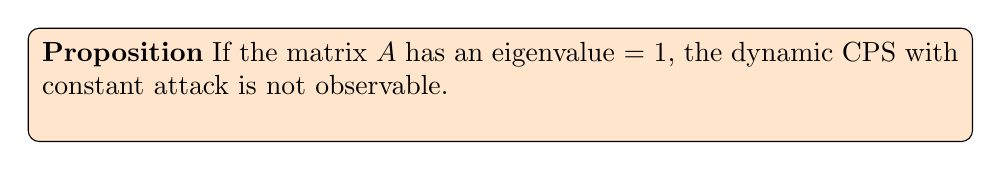
\begin{tikzpicture}
	\node [mybox] (box){%
		\begin{minipage}{.96\textwidth}     %Larghezza del box
			\textbf{Proposition} If the matrix $A$ has an eigenvalue = 1, the dynamic CPS with constant attack is not observable.\\
		\end{minipage}
	};
\end{tikzpicture}%

\noindent
The fact that an eigenvalue of A might be equal to one, is quite common from the moment we do not desire the situation in which the state tends to zero when $k\rightarrow\infty$.\\
Then, the proposition states that in general a CPS under attacks \textbf{is not observable} even if the attack is \textbf{constant}. However, we have not exploited yet the information about the \textbf{sparsity of the attacks} which allows us to develop a so-called \textbf{{\color{red} SPARSE OBSERVER}}. \\
Before giving the final result is useful to give a little of notation:
\begin{equation*}
	z(k) = \begin{pmatrix}
		x(k)\\a(k)
	\end{pmatrix}		\quad
	\hat{z}(k) = \begin{pmatrix}
		\hat{x}(k)\\\hat{a}(k)  
	\end{pmatrix}		\quad
	\hat{z}^{+}(k)=\begin{pmatrix}
		\hat{x}^+(k)\\\hat{a}^+(k)
	\end{pmatrix}		\quad
	G \ = \ (C \quad I)
\end{equation*}
We want to solve the problem of recover the state of the dynamic CPS under constant attacks that is to solve:
\begin{equation*}
	\min_{x\in\mathbb{R}^n, a \in \mathbb{R}^q}
	\frac{1}{2} \lVert y(k) - Gz(k) \rVert_2^2 + 
	\lambda \lVert a \rVert_1
\end{equation*}
It can be demonstrated that after a sufficient number $T$ of steps the solution is given by the following algorithm:\\

\hspace*{-5mm}
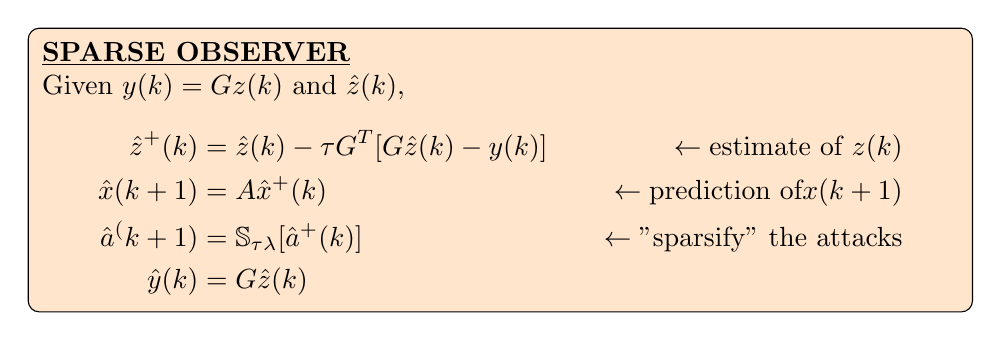
\begin{tikzpicture}
	\node [mybox] (box){%
		\begin{minipage}{.96\textwidth}     %Larghezza del box
			\textbf{\underline{SPARSE OBSERVER}}\\
			Given $y(k)=Gz(k)$ and $\hat{z}(k)$, 
			\begin{align*}
				\hat{z}^+(k)&=\hat{z}(k)-\tau G^T[G\hat{z}(k)-y(k)]
				& \leftarrow  \text{estimate of} \ z(k)\\
				\hat{x}(k+1) &= A\hat{x}^+(k) 
				 & \leftarrow \text{prediction of} x(k+1) \\
				 \hat{a}^(k+1) &= \mathbb{S}_{\tau\lambda}[\hat{a}^+(k)]
				 & \leftarrow \text{"sparsify" the attacks}\\
				 \hat{y}(k) &=G\hat{z}(k)
			\end{align*} 			
		\end{minipage}
	};
\end{tikzpicture}\\

\noindent
What are the differences from the previous version? The matrix $A$ is not the identity matrix, the state of the CPS \textbf{changes} $\Rightarrow$ in general $x(k) \ne x(k+1)$.


\chapter{Distributed Consensus based algorithms for CPSs}
\section{Toward the Fusion Center removal}

\section{The Consensus algorithm}

\section{Uses of the Consensus orithm}



%------------------------SECOND PART: CONTROL OF CPS---------------
\part{Control of Cyber-Physical systems}
\chapter{Introduction to Control of CPSs}
\section{CPSs as Multi-agent systems}
In this second part we will consider \textbf{Cyber-physical systems} as \textbf{multiagent systems} which in general can be modeled by using a directed graph (\textbf{digraph}). The figure below is an example:

\begin{figure}[h]
    \centering
    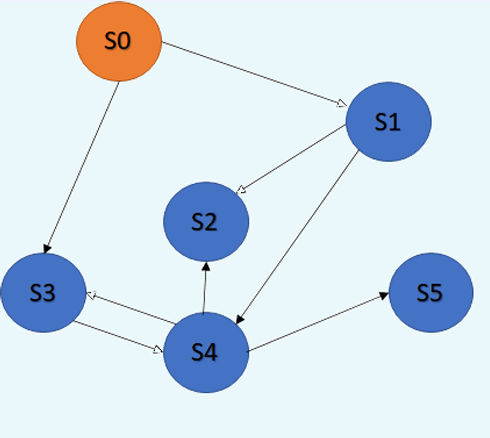
\includegraphics[scale=0.6]{images/MultiAgent.png}
    \caption{A digraph describing a multi-agent CPS}
\end{figure}

Each agent, denoted with $S_i$, can be thought as an LTI dynamical system, furthermore the digraph is used in order to represent  the \textbf{communication} among the agents which compose the \textit{overall system}.\\
In this particular \textbf{framework of multi-agent CPSs} two control problems can be recognized:
\begin{itemize}
    \itemsep0em
    \item {\color{blue}\textbf{Cooperative Tracking problem}} in which there is one \textbf{leader node}, denoted with $S_0$ and the remaing part of the nodes are N other \textbf{identical agents} which are the so-called \textbf{follower nodes}; in this type of control setting the agents \textit{cooperate} in order to follow a reference \textit{dictated by the leader node}. Examples of this approach can be: platooning, formation control and so on. {\color{red}We will focus our attention mainly on this one...} 
    \item {\color{blue}\textbf{Cooperative synchronization problem}}, the cooperation is also here in order to reach a Consensus, but in this case there is an \textbf{absence of a leader node}.
\end{itemize} 

Starting from this point we have to do an \textbf{assumption} in order to develop properly the theory:
\begin{quotation}
    \color{red}
    \textbf{Assumption} The N agents of the multi-agent system describing the CPS are \textbf{identical}, including the leader.
\end{quotation}
More later through the discussion on these topics, we will exploit a trick in order to generalize as much as possible the description of this framework.

\section{Review of LTI systems structural properties}
\noindent
Before to start talking about control algorithms and protocols can be used in the framework of multi-agent systems, it is better to retrieve and/or introduce some notions which are particularly important:
\begin{enumerate}
    \item At first a mathematical structure for the agents will be assumed (LTI systems) and some specific \textbf{structural properties} will be reminded;
    \item Then some notions on \textbf{How we can derive the mathematical model of the agents} will be given in the general framework of \textbf{black-box Error-In-Variables (EIV) System Identification}
\end{enumerate}

At the moment we can assume that the structure of the dynamical system associated to each agent $S_i$ is the Linear Time Invariant (LTI) one. Then, we can say that in the framework of \textbf{Cooperative Tracking Problem} holds that:
\begin{enumerate}
    \item The \textbf{leader node} $S_0$ is the following, at the moment we will consider that on the leader node no input is applied 
    \begin{equation}
        \begin{aligned}
            S_0: \ \begin{cases}
                \dot{x}_0=Ax_0\\
                y_0=Cx_0
            \end{cases}
        \end{aligned}
    \end{equation}
    \item The \textbf{follower nodes} $S_i, \ i=1,..., N$ are modeled as 
    \begin{equation}
        \begin{aligned}
            S_i=\begin{cases}
                \dot{x}_i=Ax_i+Bu_i\\
                y_i=Cx_i
            \end{cases}
        \end{aligned}
    \end{equation}
\end{enumerate}

At this point it is important to assume that \textbf{the triple} $(A, B, C)$ is \textbf{stabilizable} and \textbf{detectable}. 
Let us remind these important \textbf{structural properties} these dynamical systems.

\subsection{Controllabilty of an LTI system}
Roughly speaking we can say that a system is \textbf{completely (or fully) controllable} if one can \textbf{impose the behaviour} of \textbf{ALL the state variables} 'only' by acting on the inputs.  \\
Practically speaking if the system is \textit{fully controllable} then we are able to design a \textbf{state feedback} controller $K$ which is able to assign to the matrix $A-BK$ an \textbf{arbitrary} selected set of eigenvalues. We are applying to the system the law control input
\begin{equation}
    u=-Kx+\alpha r
\end{equation}

\begin{figure}[h]
    \centering
    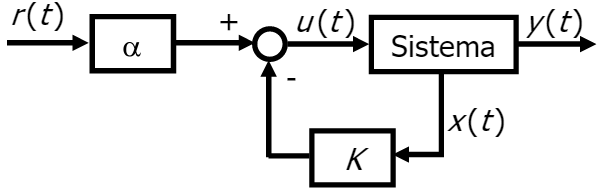
\includegraphics[scale=0.8]{images/state_feedback.png}
\end{figure}

\hspace*{-5mm}
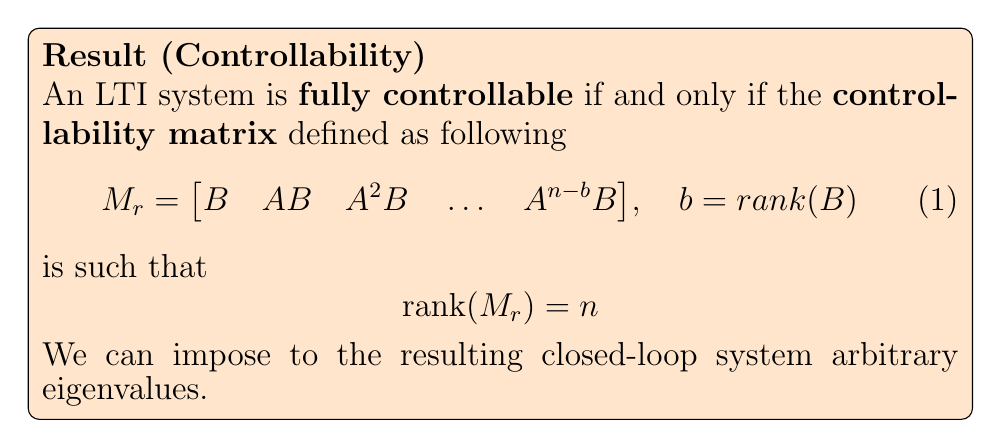
\begin{tikzpicture}
\node [mybox] (box){%
    \begin{minipage}{.96\textwidth}     %Larghezza del box
            {\large{
                \textbf{Result (Controllability)}\\
                An LTI system is \textbf{fully controllable} if and only if the \textbf{controllability matrix} defined as following
                \begin{equation}
                    M_r=\big[ B \quad 
                    AB \quad A^2B \quad \dots
                    \quad A^{n-b}B
                    \big], \quad b=rank(B)
                \end{equation}
                is such that $$\text{rank}(M_r)=n$$
                \noindent
                We can impose to the resulting closed-loop system arbitrary eigenvalues.
            }}
    \end{minipage}
};
\end{tikzpicture}%

\vspace{0.2cm} \noindent
\textbf{What happens if the system is not fully controllable}? This is equivalent to state that rank($M_r$)=$\rho<n$ and so we can only impose $\rho$ out of $n$ eigenvalues by design a proper state feeedback matrix $K$, while $n-\rho$ eigenvalues cannot be modified. Two major situations can occur:
\begin{itemize}
    \item[(A)] The $n-\rho$ eigenvalues have \textit{real part} which is strictly negative $\iff$ the system is {\color{red}\textbf{stabilizable}  }.
    \item[(B)] The remaining $n-\rho$ eigenvalues have real part which is greater or equal than zero $\iff$ the system is \textbf{not stabilizable}.
\end{itemize}

\noindent
We have just understood that when the fully controllability property is not respected the LTI system $\mathcal{S}$ can be divided into two parts:
{\large{
    \begin{equation*}
        \mathcal{S}=\begin{cases}
            \text{controllable part }&\to {\rho \ \text{eigenvalues}}\\
            \text{non-controllable part}&\to {n-\rho \ \text{eigenvalues}}
        \end{cases}
    \end{equation*}
}}

\subsection{Observability of an LTI system}
Roughly speaking we can say that an LTI system is \textbf{completely (or fully) observable} if and only if the behaviour  of \textit{all the state variables} can be \textbf{reconstructed} by only measuring the outputs. This is equivalent to state that \textbf{each variable has an effect on the output}.\\
Practically speaking, if the system if \textit{fully observable}, then we can \underline{always} design a device called (in general) \textbf{Luemberger Observer} which is able to provide an \textbf{estimate} asymptotically convergent of all the state variables by only \textbf{exploiting the information} provided by the inputs and the outputs.  

\begin{figure}[h]
    \centering
    \includegraphics[scale=0.8]{images/observer.png}
\end{figure}

Then, the \textbf{observer} is useful for  designing a feedback controller when we can only measure $y$ and not the entire \textbf{state vector}.
In order to be more specific, on such aspect, if the system is \textbf{fully observable}, then we can always find the \textbf{observer gain matrix} $L$, to arbitrarily assign the eigenvalues of the matrix $A-LC$, which describe the dynamics of the \textbf{estimation error}. \\

\hspace*{-5mm}
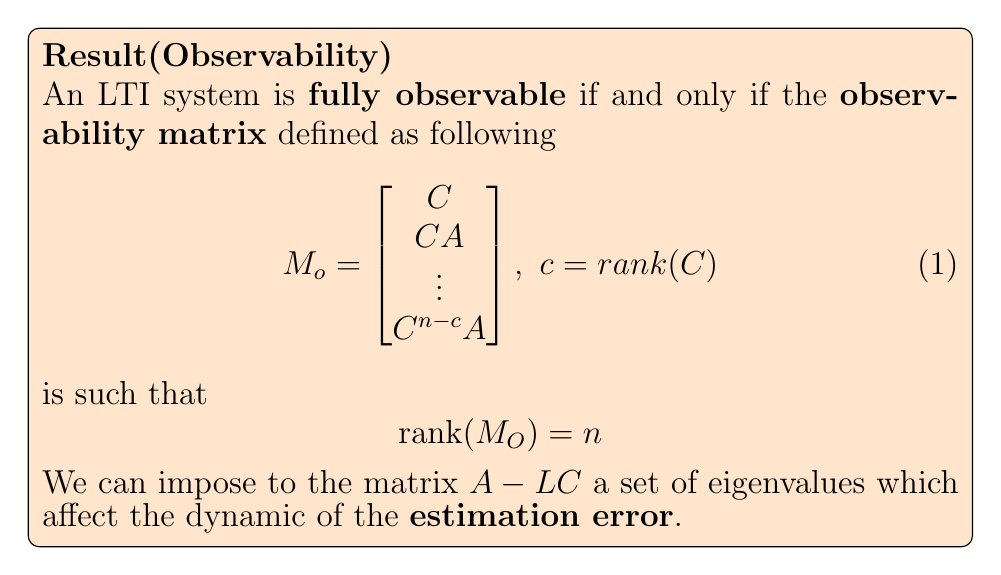
\begin{tikzpicture}
\node [mybox] (box){%
    \begin{minipage}{.96\textwidth}     %Larghezza del box
           {\large{
            \textbf{Result(Observability)}\\
            An LTI system is \textbf{fully observable} if and only if the \textbf{observability matrix} defined as following
            \begin{equation}
                M_o=\begin{bmatrix}
                    C\\CA\\\vdots\\C^{n-c}A
                \end{bmatrix}, \ c=rank(C)
            \end{equation}
            is such that 
            $$\text{rank}(M_O)=n$$
            We can impose to the matrix $A-LC$ a set of eigenvalues which affect the dynamic of the \textbf{estimation error}.
           }}
    \end{minipage}
};
\end{tikzpicture}%

\vspace{0.2cm}
\noindent
\textbf{What is happening if the system is not fully observable?} For sure we can state that rank($M_O$)=$\gamma<n$, so we can impose only $\gamma$ eigenvalues to the matrix $A-LC$. \\
The remaining $n-\gamma$ eigenvalues can be such that:
\begin{itemize}
    \item[(A)] Their real part is \textbf{strictly negative}, in this case we say that the system is {\color{red}\textbf{detectable}}. Otherwise
    \item[(B)] If at least one eigenvalue, among the $n-\gamma$ which are not observable, is null or positive, the system is \textbf{not detectable}.
\end{itemize} 
Similarly than the controllability, also in this case we can decompose the system into two other parts:
{\large{
    \begin{equation*}
        \mathcal{S}=\begin{cases}
            \text{observable part }&\to {\rho \ \text{eigenvalues}}\\
            \text{non-observable part}&\to {n-\rho \ \text{eigenvalues}}
        \end{cases}
    \end{equation*}
}}
\noindent
It is important to remember that:
\begin{quote}
    \color{red}
    Any control technique can work only with the parts \textbf{controllable} and \textbf{observable} of the system $\mathcal{S}$. The remaining \textit{non-observable} and \textit{non-controllable} part have to be \textbf{asymptotically stable}, otherwise whatever is the control method used, those part cannot be modified.
\end{quote}



\noindent
{\color{blue}\textbf{Remark (Transfer function description)}}  Note that we are focusing on the \textbf{state-space description} because the tractation we will do is essentially based on this type of model, BUT without loss of generalities, we might use also the description by mean of the \textbf{transfer function}. Because:
\begin{enumerate}
    \item If the system $\mathcal{S}$ is fully observable and controllable, the \textbf{poles} of the transfer function $H(s)$ or $H(z)$ are the eigenvalues of the system;
    \item If the system is neither fully observable nor controllable, the \textbf{poles of the transfer function} are a subset of the eigenvalues of the system, and in particular whose related to the controllable and observable part.
\end{enumerate}
We can obtain from the state-space representation the transfer function directly by applying the \textbf{Laplace transform}, the inverse step can be done by using the properties of the \textbf{realizability theory}, this frees us to use other types of techniques frequency-based  such as \textit{loop-shaping}, LQR, $\mathcal{H}_\infty$ synthesis and so on.

\section{The communication network through a digraph}
\noindent
We have mentioned that the communication among the agents is modeled by mean of a directed graph. Let us give some more details which are useful when some control algorithms and synchronization protocols are formalized.\\
\noindent
The communication network among the agents is represented by the digraph
{\large{
    \begin{equation}
        \mathcal{G} = \{\mathcal{V}, \mathcal{E}\}, \ \mathcal{V}=\{v_1, v_2, ..., v_N\}, \ 
        \mathcal{E} \subset \mathcal{V} \times \mathcal{V}
    \end{equation}
}}
However, when we treat the \textbf{synchronization problem} it is useful include in the vertices set $\mathcal{V}$ also the vertex associated to the \textit{leader node} obtaining an \textbf{augmented graph}
{\large{
    \begin{equation}
        \bar{\mathcal{G}} = \{
            \bar{\mathcal{V}}, \bar{\mathcal{E}}
        \}, \ 
        \bar{\mathcal{V}}=\{v_0, v_1, ...,v_N\}, \ 
        \bar{\mathcal{E}}=\bar{\mathcal{V}} \times \bar{\mathcal{V}}
    \end{equation}
}}


\chapter{Experimental modeling of the agents: System identification}
The focus of this chapter is on the problem of \textbf{deriving a mathematical model} of $N$ identical LTI agents $S_i$, $i=1,...,N$. The agents can be described:
\begin{itemize}
    \itemsep0em
    \item In the \textbf{Discrete Time Domain} ($t\in\mathbb{R}^+$):
    \begin{align*}
        &\text{state-space description} &\quad
        &\begin{cases}
            \dot{x}_i(t)=Ax_i(t)+Bu_i(t)\\
            y_i(t)=Cx_i(t)
        \end{cases}\\
        &\text{transfer function description} &\quad
        &H(s)=C(sI-A)^{-1}B
    \end{align*}
    \item In the \textbf{Continuous Time Domain} ($k\in\mathbb{N}$):
    \begin{align*}
        &\text{state-space description} &\quad
        &\begin{cases}
            \dot{x}_i(k)=Ax_i(k)+Bu_i(k)\\
            y_i(k)=Cx_i(k)
        \end{cases}\\
        &\text{transfer function description} &\quad
        &H(z)=C(zI-A)^{-1}B
    \end{align*} 
\end{itemize}

\section{What kind of model?}
\noindent
Different approaches are available which are based on \textbf{physical insights} and/or \textbf{input-output collected experimental data}. We can split this approaches mainly into three groups:
\begin{enumerate}
    \item \textbf{First-principle modeling}: here the structure for the system is derived only by applying the physics, moreover the equation structure is known and taken from the physic theory and, sometimes \textbf{the value of the parameter are known}, other times dedicated experiments are conducted in order to retrieve them with a certain approximation; such models are also knows as \textbf{white-box models}.
    \item \textbf{System identification}: is an approach that we find on the opposite part. In fact, here the model is derived by using \underline{\textbf{both}} input-output \textbf{collected data} and some \textbf{a-priori information} which are fundamental. The parameters come up as an \textbf{output} of the SysID procedure but do not have a physical meaning, such models bring to \textbf{black-box models}. 
    \item \textbf{Mixed approach}: here the structure of the equation is taken from the Physics (even if partially), the physical parameter to be estimated are meaningful and come up, again, as output of the procedure. The techniques which are based on these considerations are  \textbf{gray-box models}.
\end{enumerate}

\section{System Identification: black-box general setting}
\noindent
In general, the first approach which use \textbf{first-principle modeling} is not so used because the equation of the Physics are always \textit{approximation of the reality}, sometimes peculiar aspects - not trivial to mathematically formulate - can be wrongly neglected leading to bad models.\\
The \textbf{gray-box approach} is rarely used because similarly than the first case impose strong and not mild constraints on the structure of the equations and on the parameter which being related to the physical meaning cannot be arbitrarily chosen. (We will go more in details on such aspect later).\\
The most general approach is represented by the \textbf{System Identification approach} in which:
\begin{enumerate}
    \item Input-Output data are exploited, these are affected by \textit{measurement noise};
    \item Some a-priori assumption are used; 
    \item The \textbf{most natural} description, since input and output data are employed, is the \textbf{transfer function}. Finally, using the \textit{realization theory} we can obtain the state state description.
\end{enumerate}

\hspace*{-5mm}
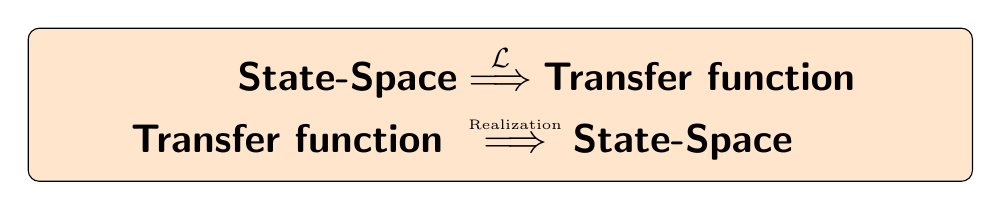
\begin{tikzpicture}
\node [mybox] (box){%
    \begin{minipage}{.96\textwidth}     %Larghezza del box
        {\Large{
            \begin{equation*}
                \begin{aligned}
                \textsf{\textbf{State-Space}}
                &\overset{\mathcal{L}}{\Longrightarrow}
                \textsf{\textbf{Transfer function }}\\
                \textsf{\textbf{Transfer function }}
                &\overset{\text{\tiny{Realization}}}{\Longrightarrow}
                \textsf{\textbf{State-Space }}
                \end{aligned}
            \end{equation*}
        }}
    \end{minipage}
};
\end{tikzpicture}%

\vspace{0.2cm}
\noindent
This approach is very used because of a \textbf{great flexibility}, for instance we need only some weak assumption based on physical insights.
Now, since the input-output data are \textbf{samples} of some signals we can start to discuss the System Identification(SysID) procedure for \textit{discrete-time systems}.\\
Without loss of generality we can say that the system to be identified (which may be in general nonlinear) can be described by using the \textit{regression form}
{\large{
    \begin{equation} \label{eq: regression_form}
        \begin{aligned}
            y(k)=&f(y(k-1), y(k-2), ...,y(k-n), \\
            &u(k), u(k-1), ..., u(k-m), \theta), \ m\le n
        \end{aligned}
    \end{equation}
}}

Where $n$ is the order of the system, while $m$ is frequently assumed to be equal to $n$. In some situation I know the value of $n$, in other situation One can choose a value for $n$ which is \textbf{sufficiently large}, then the data will guide us on the choice of the \textbf{system order}. $u(k)$ and $y(k)$ are the error-free signals.\\
A quite general setting for the SysID procedure can be surely the \textbf{Error-in-Variable (EIV)} one in which the measurement noise affects both the input and output \textbf{collected data}. 

\begin{figure}[h]
    \centering
    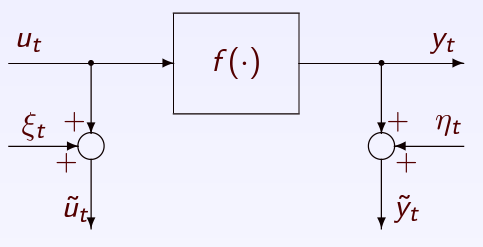
\includegraphics[scale=0.77]{images/EIV.png}
    \caption{EIV System Identification setup}
\end{figure}

\vspace{0.5cm}
%description of the terms in the figure
\noindent
How we outline before:
\begin{itemize}
    \itemsep0em
    \item[$\square$] The function $f(\cdot)$ is that to be identified;
   \item[$\square$] The terms $\tilde{u}_t$ and $\tilde{y}_t$ are the input-output collected data, which are both the real quantities ($u_t$ and $y_t$) to which is added 
   \item[$\square$] The \textbf{noise term} indicated with $\xi_t$ and $\eta_t$.
\end{itemize}

\noindent
At this point, in order to be more specific, let us clarify some aspects about the important \textbf{a-priori assumptions} which are basically of three types:
\begin{enumerate}
    \itemsep0em
    \item On which part of the system the noise enters?
    \item Assumption on the class $\mathcal{F}$ of the function $f(\cdot)$ to identify; 
    \item Is the noise of a certain type? (hypotesis on statistichal distribution, boundness, energy...)
\end{enumerate}



\subsection{Example (noise free): 2$\mathbf{^{\text{nd}}}$ order LTI system}
We have said that the most natural way to express the structure of $f(\cdot)$ is by using a \textbf{transfer function}.  But, \textbf{How can we obtain it from the regression form?} We can show it using an example.\\
Let us consider that on the system to be identified we have the following \underline{a-priori assumptions}:
\begin{enumerate}
    \item There is no noise, so $\tilde{u}_t=u_t$ and $\tilde{y}_t=y_t$;
    \item The system is \textit{linear}, in this way we have choose the class $\mathcal{F}$ for the function $f$
    \item The order of the system is $n=2$ and $m=n$.
\end{enumerate}
Using the assumption (3), the equation (\ref{eq: regression_form}), in this case becomes
\begin{equation}
    y(k) = f(y(k-1)+y(k-2)+u(k)+u(k-1)+u(k-2))
\end{equation}
Moreover, from the moment we know that the function is linear, we can express it in the following way:
\begin{equation} \label{eq: reg_linear}
    y(k)=-\theta_1y(k-1)-\theta_2y(k-2)+
    \theta_3u(k)+\theta_4u(k-1)+\theta_5u(k-2)
\end{equation}
Using the \textbf{backward shift operator} according to which $s(k-r)=q^{-r}s(k)$, we rewrite it as
\begin{align*}
    &y(k)=-\theta_1 q^{-1} y(k) -\theta_2 q^{-2} y(k) 
    + \theta_3u(k) + \theta_4 q^{-1} u(k) + \theta_5 q^{-2} u(k) \iff \\
    &y(k) +\theta_1 q^{-1} y(k) +\theta_2 q^{-2} y(k) = \theta_3u(k) + \theta_4 q^{-1} u(k) + \theta_5 q^{-2} u(k)
    \iff\\
    &y(k) [1+\theta_1 q^{-1}+\theta_2 q^{-2}] = u(k) [\theta_3+\theta_4q^{-1}+\theta_5q^{-2}] \iff\\
    & y(k) = \frac{\theta_3+\theta_4q^{-1}+\theta_5q^{-2}}{1+\theta_1 q^{-1}+\theta_2 q^{-2}} u(k)
\end{align*}
\noindent
There is a (not trivial) formal proof that the backward shift operator is equivalent to the delay $z^{-1}$ in the $\mathcal{Z}$-transform domain. It is immediate now, to find the transfer function 
\begin{equation}
    G(z) = \frac{
        \theta_3 z^2 + \theta_4z + \theta_5
    }{
        z^{2}+\theta_1z + \theta_2
    }
\end{equation}
Then, we have understood that passing through the \textit{regression form} we can obtain a \textbf{transfer function} using the a-priori assumptions and the I/O collected data.

\subsection{Estimation of the parameters}
Assuming, for the moment, we can experimentally collect I/O data without adding any noise, how can we obtain the parameters $\theta_1, ..., \theta_5$? The equation (\ref{eq: reg_linear}) have 5 unknowns, we may find a unique solution by adding other equations. \\
Before start, we have to collect a sufficient number of samples in order to compute $y(k)$, here we need the measurement $y(1), y(2), u(1), u(2)$ in order to compute $y(3)$.[In general if $n$ is the order of the system we start computing $y(k)$ from the instant $k=n+1$]. It is obtained:
\begin{align*}
    &y(3)=-\theta_1y(2)-\theta_2y(1)+\theta_3u(3)+\theta_4u(2)+\theta_5u(1)\\
    &y(4)=-\theta_1y(3)-\theta_2y(2)+\theta_3u(4)+\theta_4u(3)+\theta_5u(2)\\
    &\vdots\\
    &y(7) = -\theta_1y(6)-\theta_2y(5)+\theta_3u(7)+
    \theta_4u(6)+\theta_5u(5)
\end{align*}
that it can be rewritten in matrix form as
\begin{equation} \label{eq:sys_eq}
    \underbrace{\begin{bmatrix}
        y(3)\\y(4)\\\vdots\\y(H)
    \end{bmatrix}}_{y} 
    =\underbrace{ 
    \begin{bmatrix}
        y(2)&y(1)&u(3)&u(2)&u(1)\\
        y(3)&y(2)&u(4)&u(3)&u(2)\\
        &\vdots&\vdots&\vdots&\vdots\\
        y(H-1)&y(H-2)&u(H)&u(H-1)&u(H-2)
    \end{bmatrix}}_{A} \underbrace{\begin{bmatrix}
        \theta_1\\\theta_2\\\vdots\\\theta_H
    \end{bmatrix}}_{\theta}
\end{equation}
[In our case$H=7$]. If the matrix $A$ is invertible we can find the solution $\theta$ only by inverting the system
\begin{equation} \label{eq: inversion}
    \theta = A^{-1}y
\end{equation}
In order to guarantee that $A$ is invertible one might think that we can apply a \textit{random} input sequence, so that the columns of the matrix would be linearly independent, but it is not realistic because we want to excite the system with a particular class of signals, moreover \textbf{it is not necessary} doing such assumption: it is known what is for example the \textbf{step response} of a second-order LTI systems. There is a transient in which the output of the system oscillates a lot: 
\begin{quote}
    it is practically impossible to obtain a matrix whose columns are linearly dependent, even if the system is excited with a very simple signal of the type $u(k)=c\in\mathbb{R}$ the response has oscillations which ensure us, at a certain extent, to take independent measurements. Clearly, \textbf{the more exciting the input, the more information can be retrieved by analysing the output}.
\end{quote}

\subsection{Black-box models vs Gray-box models}
We have analysed a bit the main features of the SysID approach, so that some more specific comparison can be done with the gray-box approach.\\
The a-priori assumption on the \textit{linearity} of the system allowed us to pick a function in which \textbf{the parameters appear linearly in the model}, on the other hand their meaning is not relevant.\\
If we used more the physical insights, we are constraining the structure of the equations and so of the transfer function. For example, from the Physics one can  find that
\begin{equation*}
    G(s)=\frac{
        \sqrt{\gamma_1}s^2+\gamma_2s+\gamma_3/\gamma_4
    }{
        s^2+\frac{1}{\gamma_3}s+\gamma_5^2
    }
\end{equation*} 
Here we find that:
\begin{itemize}
    \item The \textbf{system} associated with $G(s)$ is \textbf{linear}; 
    \item The \textbf{parameters} appear in the equation \textbf{non-linearly}, and here they are meaningful because are the parameters derived from the Physics.
\end{itemize}
In general, it  is not trivial to find the solution in the case that \textbf{the system is not linear-in-parameters}, so it clearly appears that a SysID approach, without loss of generality, could bring to a simpler solution. What we lose is the meaning of the estimated parameters.

\subsection{The role of the a-priori information}
Introducing the System Identification approach, we have remarked that is crucial that \textit{collected data} and \textit{a-priori assumption} are used in order to estimate the parameters. \textbf{What if we do not use the physical insights to retrieve the structure of the system?} Let us give an example for a \textbf{static} and \textbf{non-linear} system.
\begin{equation*}
    y(k)=\theta_1u(k) + \theta_2 u(k)^2 + \theta_3 u(k)^3 + \theta_4 u(k)^4 + \theta_5 u(k)^5
\end{equation*}
Even if the equation linked to the system is \textbf{non-linear}, the parameters appear \textbf{linearly} in the equation so that we can apply the same approach of the first example, we have five parameters and we need 5 equation, furthermore, since the system is static we need only 5 samples for $u$ and 5 samples for $y$:
\begin{align*}
    &y(1)=\theta_1 u(1)+ \dots + \theta_5 u(1)^5\\
    &y(2)=\theta_2 u(2)+ \dots + \theta_5 u(2)^5\\
    &\vdots \quad = \quad \quad \vdots \\
    &y(5)=\theta_2 u(5) + \dots + \theta_5 u(5)^5
\end{align*}
\noindent
That in matrix form
\begin{equation*}
    \begin{bmatrix}
        y(1)\\y(2)\\\vdots\\y(5)
    \end{bmatrix}=\begin{bmatrix}
        u(1)&u(1)^2&...&u(1)^5\\
        u(2)&u(2)^2&...&u(2)^5\\
        \vdots&\vdots&\vdots&\vdots\\
        u(5)&u(5)^2&...&u(5)^5
    \end{bmatrix} \begin{bmatrix}
        \theta_1\\\theta_2\\\vdots\\\theta_5
    \end{bmatrix}
\end{equation*}
If we invert the system by applying the equation (\ref{eq: inversion}) we will obtain the parameter $\theta$, BUT \textbf{what if we use the resulting $y(k)$ to predict the behaviour of the system?} We neglected the relevant fact the system is of the second order! At this point:
\begin{enumerate}
    \item If we use the collected data to do the prediction, it will be correct for sure \textbf{(we built the model relying only on them)}
    \item If we apply a certain sequence $u(k)$ to the system $\mathcal{S}$ and we take the corrensponding $y(k)$ samples, we will note that the prediction done according to the identified model is \textbf{completely wrong!}.
\end{enumerate}
Conclusion:
\begin{quote}
    \large{\color{blue}
        In the System Identification procedure if we rely only on the input-output collected data, we will \textbf{overfit} the data, this is the reason why \textbf{the a-priori assumptions act a fundamental role in the identification procedure}.
    }
\end{quote}


\subsection{From the ideal situation to the real experiment}
Only in order to simplify the explanation, we started with the assumption that the input-output collected data were \textbf{noise-free}. In the real-world experiments we cannot do this assumption! Always we have that the collected data is:
\begin{align}
    &\tilde{u}_t = u_t+\xi_t\\
    &\tilde{y}_t = y_t+\eta_t
\end{align}
Making us guided from an example, this situation will be more clear. Let us consider a very simple  example: a \textbf{resistor} through which a current $i(t)$ is passing. The input $u(t)$ is the current $i(t)$ itself, while the output is clearly the voltage $v(t)$ on the resistor. The simple equation which describe this system is 
\begin{equation}
    y(k) = \theta u(k)
\end{equation}
Following the procedure we did before and considering that only the output $\tilde{y}(k)$ is affected by the noise, we have a \textbf{single parameter}; then a single equation, and a \textbf{single sample} to be taken of the input and the output, might be sufficient in order to obtain an \textbf{estimate} $\hat{\theta}$ of the parameter, which in this case we know that is a \textbf{resistance}.
If we had used the real $u(k)$ and $y(k)$, the $\theta$ parameter would have been
\begin{equation}
    \theta = \frac{y(k)}{u(k)}
\end{equation}
but, if we apply our naive approach using the collected data which are corrupted by the \textbf{measurement noise} we obtain
\begin{equation}
    \hat{\theta} = \frac{\tilde{y}(k)}{u(k)} = 
    \frac{y(k)}{u(k)}+\frac{\eta{k}}{u(k)} = \theta + \frac{\eta(k)}{u(k)} \ne \theta
\end{equation}
Conclusion:
\begin{quotation}
    If we use a single sample, we will obtain for sure a wrong estimate of the single parameter $\theta$ $\to$ a \textbf{wrong model}. We need more samples and we will look for a $\theta$ which is providing the \textbf{best-fitting} of the data.
\end{quotation}

\noindent
In order to exit from this \textbf{wrong situation}, we have to collect for sure more \textit{input-output} pairs in a number $H \gg 2n+1$, where $2n+1$ given a system of order $n$ is the number of parameters to estimate $\to$ the output of our system identification procedure. However at this point we cannot apply anymore the equation (\ref{eq: inversion}) because the matrix $A$ becomes a tall matrix, which cannot be inverted! We use the Moore-Penrose pseudo inverse defined as
\begin{equation*}
    A^\dagger = (A^TA)^{-1}A^T
\end{equation*}
and we can solve the problem by simply substituting the inverse with the pseudoinverse:
\begin{equation} \label{eq: LS_solution}
    \hat{\theta} = A^\dagger y = (A^TA)^{-1}A^T y
\end{equation}
This is the solution of the Least-Squares problem (LS) to the equation (\ref{eq:sys_eq})
\begin{equation}
    \hat{\theta} = \text{arg}\min_\theta \Vert A\theta-y\Vert_2^2
\end{equation}
In this way $\hat{\theta}$, in the context of System Identification, is the LS estimate of the \textit{parameter vector}.\\
This formulation of the problem has interesting properties if some hypothesis are satisfied:
\begin{enumerate}
    \item The error apper in the equation as an additive term $e(k)$ called the \textbf{equation error}; 
    \item The $e(k) k=1,...,H$ represents a white gaussian noise, that is the samples are \textit{indipendent and identically distributed} (iid).
\end{enumerate}
If such assumption are fullfilled, then
{\large{
    \begin{equation}
        \lim_{H\to\infty} \mathbb{E}\big[\hat{\theta}\big] = \theta
    \end{equation}
}}
Where $\theta$ is the \textbf{true parameter vector}. The Least Square approach, no matter what are the dimension of the matrix is \textbf{very fast}, moreover there is also an \textit{online recursive way} to compute them.\\
At this point we are assuming that:
\begin{align*}
    &y(k)=-\theta_1y(k-1)-\theta_2y(k-2)-...-\theta_ny(k-n)+\theta_{n+1}u(k)+...+\theta_{n+m+1}u(k-m) + e(k) \iff \\
    &y(k)=-\theta_1 q^{-1}y(k)-\theta_2 q^{-2}y(k)-...-\theta_n q^{-n}y(k) + \theta_{n+1}u(k) + ... + \theta_{n+m+1} q^{-(n+m+1)} u(k) + e(k) \iff \\
    &y(k) \big(1+\theta_1 q^{-1}+...+\theta_n q^{-n} \big) = u(k) \big( \theta_{n+1} q^{n+1}+...+\theta_{n+m+1}  q^{n+m+1} \big) + e(k) \iff \\
    &y(k) D_d(q^{-1})=u(k)\ N_d(q^{-1}) + e(k) \iff 
    y(k)=\frac{N_d(q^{-1})}{D_d({q^{-1}})} u(k) + \frac{1}{D_d(q^{-1})}e(k) \quad _\blacksquare
\end{align*}
This last step we did tells us that the output of the system \textbf{to be identified} depends:
\begin{enumerate}
    \item On the transfer function to be identified $\frac{N_d(q^{-1})}{D_d({q^{-1}})}$ (this is ok);
    \item On the error filtered by the transfer function $\frac{1}{D_d(q^{-1})}$ which depends directly on something to be identified  yet!
\end{enumerate}

\noindent
\textbf{Conclusion}
The Least-Squares estimator used to solve the SysID problem has some advantages: fast convergence and simplicity, however in order to be used requires \textbf{strong assumption} on the error, moreover even if this can be obtained, having an acceptable estimate requires the collection of a big quantity of data. 
\begin{center}
    \color{red}
    We need an approach where:
    \begin{enumerate}
        \item A \textbf{small amount of data} is required; 
        \item \textbf{mild assumption} on the error has to be done.
    \end{enumerate}
    These needs leads to the \textbf{Set-Membership System Identification} theory.
\end{center}


  








\chapter{Set-membership System Identification}
The main motivation which leads us to look for another approach to be used is that we want to:
\begin{enumerate}
    \itemsep0em
    \item Use a small amount of data
    \item Have \textit{mild} assumptions on the noise.
\end{enumerate}

\section{Main ingredients}
In order to formulate the \textbf{Set-Membership System Identification problem} we need some important ingredient:
\begin{itemize}
    \itemsep0em
    \item We start from a discrete time \textit{parametrized regression form} 
    \begin{equation*}
        y(k) = f(y(k-1),...,y(k-n), u(k), u(k-1), u(k-m), \theta_1, ..., \theta_{n+m+1}), \quad m \le n
    \end{equation*}
    \item A-priori assumptions on the \textbf{system} $\mathcal{S}$:
    \begin{itemize}
        \item $m,n$ are known; 
        \item The function $f\in\mathcal{F}$ (for the moment we choose the LTI class of dynamical systems).
    \end{itemize}
    \item A-priori assumptions on the \textbf{noise}:
    \begin{itemize}
        \item Noise structure (\textbf{OE, EIV}); 
        \item The input and output noise is part of some \textbf{bounded sets} $\mathcal{B}$ and in particular:
        {\large{
            \begin{align*}
                &\eta(k)\in\mathcal{B}_\eta, \quad
                \xi(k) \in \mathcal{B}_\xi
            \end{align*}
        }}
    \end{itemize}
    Tipically the sets $\mathcal{B}$ are defined by \textbf{polynomial constraints}, it is common that
    {\large{
        \begin{equation*}
            \mathcal{B}_\eta = \{
                \eta: \ \vert \eta(k) \vert \le \Delta_\eta
            \}, \quad
            \mathcal{B}_\xi = \{
                \xi : \ \vert \xi(k) \vert \le \Delta_\xi
            \}
        \end{equation*}
    }}
\end{itemize}

The \textbf{key element} of the Set-Membership identification method is the research of the \textbf{Feasible parameter set (FPS)} that we denote with $\mathcal{D}_\theta$. In a nutshell, it is the set of the parameter $\theta$ such that all the conditions exposed are fullfilled.

\section{Noise structures}

\subsection{Error-In-Variable set-up (EIV)}
\begin{figure}[h]
    \centering 
    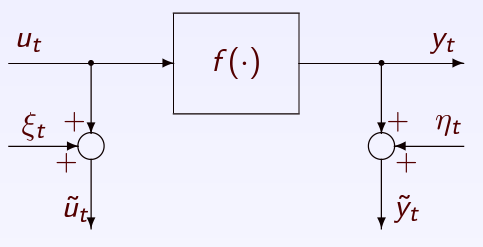
\includegraphics[scale=1]{images/EIV.png}
    \caption{EIV set-up}
\end{figure}
\textbf{Error-In-Variables (EIV)} problem refers to the most general case where the measurement noise is added both in the input and the output.\\
Due to the conditions we mentioned, we  have that:
{\large{
    \begin{equation*}
        \xi = [\xi(1) \quad ... \quad \xi(H)]\in \mathcal{B}_\xi, \quad
        \eta = [\eta(1) \quad ... \quad \eta(H)]\in \mathcal{B}_\eta
    \end{equation*}
}}

\subsection{Output-Error set-up(OE)}
\textbf{Output-Error(OE)} problem arises when the measurement noise $\eta$ enters only on the output of the system, while the system is assumed to be \textbf{exactly known}. [This is not strange to assume because sometimes one build the sequence of input to stimulate the system]. \\
Due to the condition we mentioned, we have that:
{\large{
    \begin{equation*}
        \eta = [\eta(1) \quad ... \quad \eta(H)]\in\mathcal{B}_\eta
    \end{equation*}
}}
\begin{figure}[h]
    \centering
    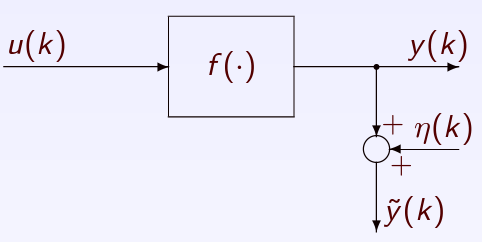
\includegraphics[scale=1]{images/OE.png}
    \caption{OE set-up}
\end{figure}

\section{Feasible Parameter Set (FPS)}
In the framework of \textbf{Set-Membership(SM) Identification}, all the parameters values consistent with the (i) \textit{a-priori information on the model}, (ii) \textit{a-priori information on the noise}, (iii) collected input/output data are considered as:
\begin{center}
    \large
    Feasible solution of the system identification problem
\end{center}
The set of all the parameters which satisfies these conditions is called the \textbf{Feasible Parameter Set}. For a \textbf{general EIV problem} it can be implicitly defined as:\\

\hspace*{-5mm}
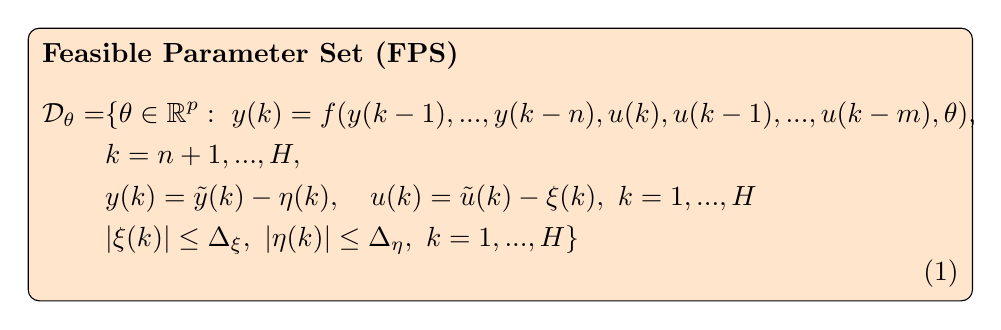
\begin{tikzpicture}
\node [mybox] (box){%
    \begin{minipage}{.96\textwidth}    
        {\normalsize{
            \textbf{Feasible Parameter Set (FPS)}\\
    \begin{equation}
        \begin{aligned} \label{eq:FPS}
            \mathcal{D}_\theta = &\{
        \theta\in\mathbb{R}^p: \
        y(k)=f(y(k-1), ..., y(k-n), u(k),u(k-1), ..., u(k-m), \theta),\\
        & k=n+1,...,H,\\
        & y(k)=\tilde{y}(k)-\eta(k), \quad 
        u(k)=\tilde{u}(k)-\xi(k), \ k=1, ..., H\\
        &\vert \xi(k) \vert \le \Delta_\xi, \ 
        \vert \eta(k) \vert \le \Delta_\eta, \ 
        k=1,...,H
        \}
        \end{aligned}
    \end{equation}
}}
    \end{minipage}
};
\end{tikzpicture}%

\noindent
In the case that we want to identify a LTI discrete time system the set (\ref{eq:FPS}) is:
{\large{
    \begin{equation}
        \begin{aligned}
            \mathcal{D}_\theta =&\{
                \theta\in\mathbb{R}^p: \ 
                (\tilde{y}(k)-\eta(k))+
                \sum_{i=1}^n {\theta_i (\tilde{y}(k-1)-\eta(k-1))} =\\ &=\sum_{j=0}^m {\theta_j} (u(k-j)-\xi(k-j)), \ k=n+1, ..., H \\
                &\vert \xi(k) \vert \le \Delta_\xi, \ 
                \vert \eta(k) \vert \le \Delta_\eta, \ 
                k=1,...,H
            \}
        \end{aligned}
    \end{equation}    
}}

\noindent
The \textit{Feasible Parameter Set} enjoys the following properties:
\begin{enumerate}
    \itemsep0em
    \item The \textit{true value} of the parameter vector $\theta$ is guaranteed to belong to $\mathcal{D}_\theta$; 
    \item $\mathcal{D}_\theta$ implicitly quantify the uncertainty affecting the found mathematical model.
\end{enumerate}

Once we have found the FPS, we can use it to find \textbf{for each parameter} $\theta_k$ the \textit{Parameter Uncertainty Interval (PUI)} which is formally defined as
{\large{
    \begin{align}
            &PUI_k = [\underline{\theta}_k;\ \overline{\theta}_k], \\
        &\underline{\theta}_k=\min_{\theta\in\mathcal{D}_\theta} {\theta_k}, \quad \overline{\theta}=\max_{\theta\in\mathcal{D}_\theta} {\theta_k} \label{eq:PUIs}
    \end{align}
}}
The computation of $PUI_k$ requires to compute the \textbf{global optimal solution} of the optimization problems in (\ref{eq:PUIs}).

\subsection{Example \#1}
Let us suppose that the model to identify is a static system: a resistor.

\subsubsection{Ingredients}
\begin{enumerate}
    \item \textsc{A-priori information on the system}: $y(k)=\theta u(k)$
    \item \textsc{A-priori information on the noise} here we assume a \textbf{OE} noise structure, where $\vert \eta(k) \vert \le \Delta\eta$
    \item \textsc{A-posteriori info (I/O collected data)}, I have the pairs $[u(k), \tilde{y}(k)], k=1,...,H$
\end{enumerate}

\subsubsection{Feasible Parameter Set Computation}
{\large{
    \begin{align*}
        &\begin{aligned}
            \mathcal{D}_\theta = &\{
                \theta \in \mathbb{R}: y(k)=\theta u(k) \forall k=1,..., H \\
                &y(k)=\tilde{y}(k)-\eta(k), \quad \forall k=1,...,H\\
                &\vert \eta(k) \vert \le \Delta_\eta
            \}\Longleftrightarrow
        \end{aligned}\\ 
        &\begin{aligned}
            \mathcal{D}_\theta = &\{
                \theta \in \mathbb{R}: \tilde{y}(k)-\eta(k)=\theta u(k), \quad
                \vert \eta(k) \vert \le \Delta_\eta, \ 
                k=1,...,H 
            \}
        \end{aligned}\\
        &\begin{aligned}
            \mathcal{D}_\theta = &\{
                \theta \in \mathbb{R}: \eta(k)=\tilde{y}(k)-\theta u(k), \quad
                \vert \eta(k) \vert \le \Delta_\eta, \ 
                k=1,...,H 
            \}
        \end{aligned}\\
        &\begin{aligned}
            \mathcal{D}_\theta = \{
                \theta \in \mathbb{R}: \
                -\Delta_\eta \le \tilde{y}(k)-\theta u(k) \le \Delta_\eta, \quad
                k=1,...,H
            \}
        \end{aligned}\\
        &\begin{aligned}
            \mathcal{D}_\theta = \bigg\{
                \theta \in \mathbb{R}: \ 
                \theta \ge \frac{\tilde{y}(k)-\Delta_\eta}{u(k)}, \ \theta \le \frac{\tilde{y}(k)+\Delta_\eta}{u(k)}, \quad \forall k=1,...,H
            \bigg\}
        \end{aligned}
    \end{align*}
}}
In this case the FPS is the intersection between $H$ intervals, and the $PUI$ for the only parameter $\theta$ is coincident with this found interval.
We succeded in eliminating the dependence on $\xi,\eta$, but this was only  a particular case.\\
If only the system to identify had been only a little bit more complicated, the trick we used to eliminate $\eta$ from the set, would not have work. 

\section{Extended Feasible Parameter Set (EFPS)}
\noindent
This fact highlight the necessity to enlarge the FPS in such a way, it is able to contain also the variable $\theta, \xi$ which depends on the input and output error, defining the \textbf{Extended Feasible Parameter Set (EFPS)}.\\

\hspace*{-5mm}
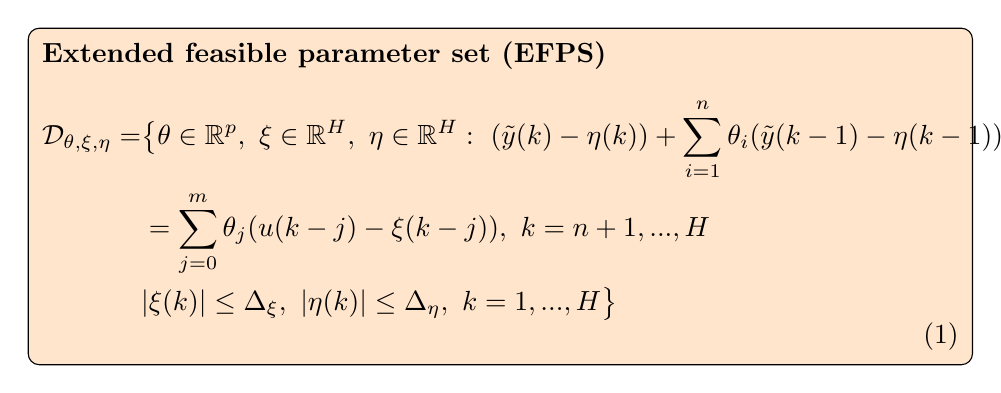
\begin{tikzpicture}
\node [mybox] (box){%
    \begin{minipage}{.96\textwidth}     %Larghezza del box
        {\normalsize{
            \textbf{Extended feasible parameter set (EFPS)}\\
            \begin{equation}
                \begin{aligned}
                    \mathcal{D}_{\theta,\xi,\eta} =&\big\{
                        \theta\in\mathbb{R}^p,\ 
                        \xi \in \mathbb{R}^H, \
                        \eta \in \mathbb{R}^H: \ 
                        (\tilde{y}(k)-\eta(k))+ 
                        \sum_{i=1}^n {\theta_i (\tilde{y}(k-1)-\eta(k-1))} =\\ &=\sum_{j=0}^m {\theta_j} (u(k-j)-\xi(k-j)), \ k=n+1, ..., H \\
                        &\vert \xi(k) \vert \le \Delta_\xi, \ 
                        \vert \eta(k) \vert \le \Delta_\eta, \ 
                        k=1,...,H
                    \big\}
                \end{aligned}
            \end{equation} 
        }}
    \end{minipage}
};
\end{tikzpicture}%

This is the set of the parameters $\theta$ and noise samples $\xi, \eta$ which are consistent with the \textit{a-priori assumptions}. The FPS $\mathcal{D}_\theta$ we defined in the previous paragraphs is only the projection in the parameter space $\mathbb{R}^p$ of the EFPS $\mathcal{D}_{\theta,\xi,\eta}$.
Moreover the PUIs have to be computed on the extended space that in general is a \textbf{non-convex set} defined by \textbf{polynomial constraints}, in the following way:
{\large{
    \begin{equation}
        \underline{\theta}_k=\min_
        {\theta,\xi,\eta\in\mathcal{D_{\theta,\xi,\eta}}} {\theta_k}, \quad \overline{\theta}=\max_{\theta,\xi,\eta\in\mathcal{D_{\theta,\xi,\eta}}} {\theta_k} \label{eq:PUIs}
    \end{equation}
}}
One can wonder how to use the PUI for each parameter once you found it.  Usually for each $PUI_k$, the best choice is the \textbf{central estimate} $\theta_c$ defined as
\begin{equation*}
    \theta_{c,k} = \frac{\underline{\theta}_k+\overline{\theta}_k}{2}
\end{equation*}
By doing an example, there will be the possibility to better clarify some aspects even on the EFPS, that on the \textbf{central-estimate}, this gives us also the possibility to introduce some other theoretical aspects. 

\subsection{Example: First order system} 
Let us consider the problem of identifying a \textbf{first order system} of the form: 
\begin{equation*}
    y(k) = -\theta_1 y(k-1) + \theta_2 u(k)
\end{equation*}
The EFPS for such system is as following:
\begin{align*}
    \mathcal{D}_{\theta, \xi, \eta} = \big\{
        \theta \in \mathbb{R}^2, \xi \in \mathbb{R}^H, \eta \in \mathbb{R}^H: \ 
        &\tilde{y}(k)-\eta(k) = -\theta_1 \tilde{y}(k-1) + \theta_1 \eta(k-1) + \\
        &\theta_2 \tilde{u}(k) - \theta_2\xi(k) \forall k=2,..., H\\
        & \vert \eta(k) \vert \le \Delta_\eta, \ 
        \vert \xi(k) \vert \le \Delta_\xi
    \big\}
\end{align*}
We can note that the equations are exactly the same, with the difference that the FPS $\mathcal{D}_\theta$ is a \textbf{projection} of the EFPS onto the \textbf{parameter space}.
This set is characterized by: 
\begin{itemize}
    \itemsep0em
    \item nonlinear \textbf{equality constraints}, in particular they are bilinear and in general non-convex!
    \item \textbf{linear inequality constraints}
\end{itemize}
The projection of the EFPS on $\mathcal{D}_\theta$ is a non-convex set which can have some strange shape. The figure below constitutes an example of the FPS for the proposed Set-Membership identification problem. The extremities of each $PUI$ is depicted. In this way we have obtain the minimum (2D) hyper-rectangle which contains the Feasible Parameter Set.

\begin{figure}[h]
    \centering 
    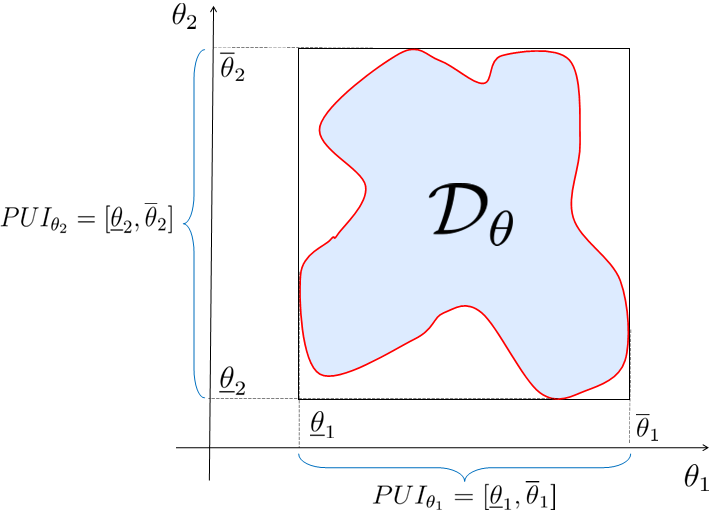
\includegraphics[scale=0.8]{FPS.png}
    \caption {FPS for a first order SysID problem}
\end{figure}
\noindent
After having completed the computation of the Parameter uncertainty intervals for all $\theta_k$, we can derive using the \textit{backward-shift operator} and the $\mathcal{Z}$-transform the \textbf{transfer function} of the agent
\begin{align*}
    G(z) &= \frac{\theta_2 z}{z+\theta_1}\\
    &  \text{where} \quad \theta_1 \in [\ \underline{\theta}_1, \ \overline{\theta}_1 \ ], \ \theta_2 \in [\ \underline{\theta}_2, \ \overline{\theta}_2 \ ]
\end{align*}
It is remarkable that for each point inside the set in blue we have a \textbf{different model}, but one can wonder: \textbf{How can we use this $PUI$?}
\begin{enumerate}
    \item If we are going to apply either robust control or robust simulation (for example using $\mathcal{H}_\infty, \mu$-synthesis and so on), this modelis already in the \textbf{correct form}!
    \item In other situations we would like to find a \textbf{single model} inside $\mathcal{D}_\theta$ to be used as the "best" (or \textbf{nominal model}). That is, we need to find a rule for selecting a single value of $(\theta_1, \theta_2)$ one single point inside the blue region. In this case it is a common choice to pick \textit{for each PUI} the \textbf{central estimate}
    {\large{
        \begin{equation*}
            \theta_k^c = \frac{\underline{\theta}_k+\overline{\theta}_k}{2}
        \end{equation*}
    }}
    \noindent
    this represents the center of the hyper-rectangle inside which the FPS lies. More rigorously, we define the \textbf{central estimate} as the solution of the following optimization problem:
    \begin{equation}
        \theta_c = \min_{\theta\in\mathbb{R}^2} \max_{\theta'\in\mathcal{D}_\theta} \Vert \theta-\theta' \Vert_\infty
    \end{equation}
    which is also known as the \textbf{Chebyshev center of $\mathcal{D}_\theta$ in $\ell_\infty$ norm}
\end{enumerate}
[Note that... in some particular cases the FPS might be so strange that is not connected, in this course the problems which arises these cases will not be discussed.]\\
This method is guaranteed to be a good choice inside the hyper-rectangle, however such center \textbf{is not guaranteed to be inside the FPS}. Consider for example the following case: 
\begin{figure}[h]
    \centering
    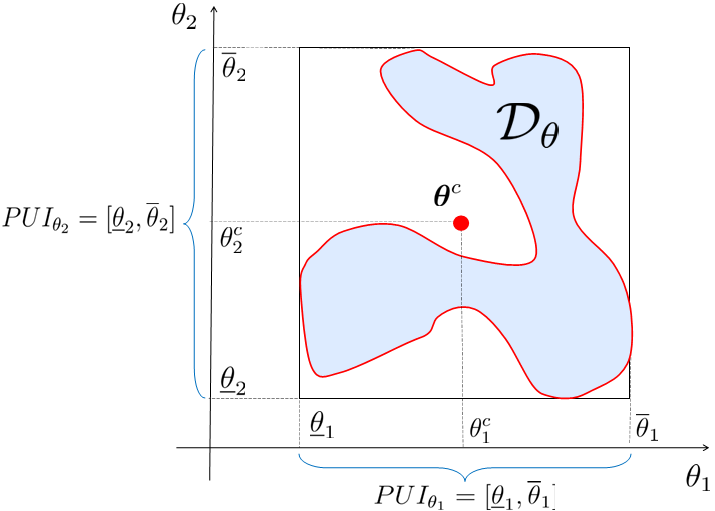
\includegraphics[scale=0.8]{FPS2.png}
    \caption{FPS with $\theta^c$ outside the set}
\end{figure}

\noindent
\textsf{[For this reason, it can be done another type of choice which is based on the use of the \textbf{conditional central estimate}, this and other related aspects are outside the purposes of this course].} 

\section{Convex relaxation for PUIs computation}
The fact that the feasible parameter set, in the most general caseof an EIV setting, is characterized by \textbf{bilinear constraints} can be used to note that \textbf{bilinearity} can be seen also as a special case of a \textbf{polynomial constraint}. We know that the FPS, as it is a projection of a non-convex set, itself it is not convex so we should solve a \textbf{non-convex optimization problem} which shows possibly a large number of local minima/maxima (optimal solution). Standard algorithm for nonlinear optimization are not able to compute the \textbf{global optimal solution}, that is the same to say that they potentially trap in local minima. \\
This is not a good news for us, since the intervals resulting from such local optimal solution cannot be qualified as PUIs, because it is not guaranteed that we can find $\theta_{\text{true}}$ inside them.\\

For the specific class of polynomial optimization problem (POP), powerful results are available to compute the solution which are based on the \textsf{Moment Theory} (Lassere). This tool can turn the original non-convex problem into a sequence of Semidefinite Programs (SDP) which instead are \textbf{convex}, their size depends on a parameter $\delta$ which is called the relaxation order.

The method is based on finding a convex approximation $\mathcal{D}^\delta_\theta$ for the FPS which is able to contain it. The higher the relaxation order $\delta$, the better the approximation. \\
It can be proved that when $\delta\to\infty$ a \textbf{convex hull} is obtained which is qualified as the smallest convex set which contains our (non-convex) FPS.

\begin{figure}[h]
    \centering
    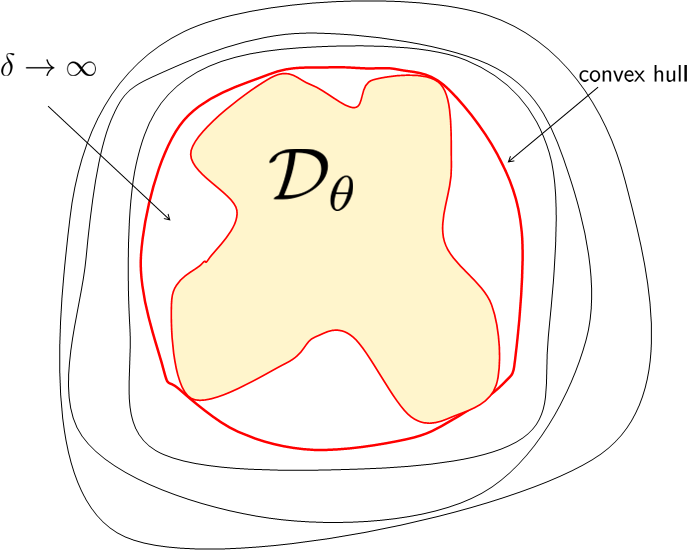
\includegraphics[scale=0.7]{relaxation.png}
\end{figure}


\noindent
The relaxation order has to have a minimum value which is:
\begin{equation}
        \delta_{min} = \max \bigg[
            \frac{deg(f_k(x))}{2}
    \bigg]
\end{equation}
where $f_k(x)$ are the constraints of the optimization problem. 
For any relaxation order $\delta$ which satisfies the constraint above, which is $\delta \ge \delta_{min}$ it is guaranteed that:
\begin{align*}
    \underline{\theta}_k^\delta \le \underline{\theta}_k, \quad 
    \overline{\theta}_k^\delta \ge \overline{\theta}_k \quad \forall k=1,...,n+m+1 
\end{align*}
Moreover it holds that:
{\Large{
    \begin{equation}
        \lim_{\delta\to\infty}  \underline{\theta}_k^\delta = \underline{\theta}_k, \quad
        \lim_{\delta\to\infty} \overline{\theta}_k^\delta = \overline{\theta}_k
    \end{equation}
}}
A \textbf{big disadvantage} of such relaxation method is the \textbf{computational complexity} that in particular grows exponentially in the relaxation order $\delta$. Therefore, the problem is tractable only in the case that $\delta$ is small. \\
The convex relaxation technique can be applied by using the freely available MATLAB tool \texttt{SparsePOP}. Given a POP, this tool automatically computes the convex SDP relaxation for a given relaxation order $\delta$. Finally, \texttt{SparsePOP} calls another software which is called \texttt{SeDuMi} in order to \textit{solve the SDP problems} obtained by convex relaxation.

\subsection{Solution of a generic POP using \texttt{SparsePOP}}
The tool \texttt{SparsePOP} is able to solve any optimization problem like:
{\large{
    \begin{align*}
        \min_{x\in\mathbb{R}^n}  \quad & f_0(x)\\
        &\text{s.t.}\\
        &f_k(x)\ge 0 \quad (k=1,...,l)\\
        &f_k(x)=0 \quad (k=l+1, ..., m)\\
        &\texttt{lb}_i \le x_i \le \texttt{ub}_i
    \end{align*}
}}
where $f_0,...,f_k$ are \textit{multivariate polynomial} function of the optimization variable $x\in\mathbb{R}^n$.
Let us introduce some examples in order to show how \texttt{SparsePOP} formulates the optimization problems, particular data structures has to be introduced for this aim.

\subsubsection{Example \#1 (general polynomial optimization problem)}
It is given the following optimization problem:
\begin{align*}
    \min_{x\in\mathbb{R}^3} \quad &(-2x_1+ 3x_2 -2 x_3) \\
    &\text{s.t.}\\
    &6x_1^2+3x_2^2-2x^2x_3 + 3x_3^2-17x_1+8x_2-14x_3 \ge -19\\
    &x_1 + 2 x_3 + x_3 \le 5\\
    &5x_2 + 3 x_3 \le 7\\
    &0\le x_1 \le 2, \quad 0 \le x_2 \le 2
\end{align*}
\noindent
\textsf{\large\textbf{SparsePOP formulation of the problem:}}\\
In the comments of the code we give some extra information, for further information see  the SparsePOP manual that is available online. \\
See: \href{URL} {https://sourceforge.net/projects/sparsepop/files/UserGuide.pdf/download}\\

\noindent
\textbf{\textsf{1) Objective function (data structures)}}

\begin{verbatim}
    objPoly.typeCone=1;         %always 1 here
    objPoly.dimVar=3;           %no opt. variables (including the constraints)
    objPoly.degree=1;           %degree of f_0
    objPoly.noTerms=3;          %number of monomials in f_0
    objPoly.supports=support;   %(matrix) see description below
    objPoly.coef=coef;          %(matrix) see description below         
\end{verbatim}
\texttt{support} and \texttt{coef} are data structures used to describe the objective function. In particular: 
\begin{itemize}
    \item \texttt{support} is a matrix with number of rows equal to \texttt{noTerms}, number of columns equal to \texttt{dimvar}, each entry of such matrix is a \textit{real number} which is the degree of the optimization variable involved in the \textbf{considered term}. In our case since we have ${f_0(x) = -2x_1+ 3x_2 -2 x_3}$ we have that \texttt{support} is equal to
    \begin{equation*}
        \texttt{support} = \begin{bmatrix}
            1&0&0\\
            0&1&0\\
            0&0&1
        \end{bmatrix}
    \end{equation*}
    it is only a case that it is an identity matrix.
    \item \texttt{coef} is a \textit{column vector} with coefficient of the different terms involved in $f_0(x)$. In our case we have that: 
    \begin{equation*}
        \texttt{coef} = \begin{bmatrix}
            -2\\3\\2
        \end{bmatrix}
    \end{equation*}
\end{itemize}

\noindent
\textbf{\textsf{2) Constraints (data structures)}}\\
The data structures related to the constraints are very similar, with the only difference that we need to put inequality constraints in the form $f_k(x)\ge0$. The following data structures have to be filled \textbf{for each constraint} of the optimization problem. Finally note that, in the code, the notation \texttt{ineqPolySys{1}} denotes the part of the data structure related to the first constraint.\\
Then, let us bring the first constraint of the optimization problem in a SparsePOP-compatible form:
\begin{equation*}
    f_1(x)=19-17x_1+8x_2-14x_3+6x_1^2+3x_2^2-2x_2x_3 +3x_3^2 \ge 0 
\end{equation*}
\begin{verbatim}
    ineqPolySys{1}.typeCone=1;        % 1 if >=, -1 if =
    ineqPolySys{1}.dimVar=3;          % the same as before
    ineqPolySys{1}.degree=2;          % inequality degree (deg max of the monomials)
    ineqPolySys{1}.noTerms=8;         % no terms in the inequality
    ineqPolySys{1}.support=support;   %as before
    ineqPolySys{1}.coef=coef;         %the same as before
\end{verbatim}

\noindent
Following the fashion of the previous step, let us define \texttt{support} and \texttt{coef}: 
\begin{equation*}
    \texttt{support} = \begin{bmatrix}
        0&0&0\\1&0&0\\
        0&1&0\\0&0&1\\
        2&0&0\\0&2&0\\
        0&1&1\\0&0&2
    \end{bmatrix}, \qquad 
    \texttt{coef} = \begin{bmatrix}
        19\\-17\\8\\-14\\
        6\\3\\-2\\3
    \end{bmatrix}
\end{equation*}

\noindent
\textbf{\textsf{3) Lower and upper bounds}}\\
The lower and upper bounds are indicated by employing two vectors called \texttt{lbd} and \texttt{ubd}, where respectively \texttt{lbd}=[\texttt{lb}$_i$,...,\texttt{lb}$_\textsf{dimVar}$], \texttt{ubd}=[\texttt{ub}$_i$,...,\texttt{ub}$_\textsf{dimVar}$]. In our example:
\begin{equation*}
    \texttt{ubd} = \begin{bmatrix}
        2\\1\\1e10
    \end{bmatrix}, \quad
    \texttt{lbd} = \begin{bmatrix}
        0\\0\\-1e10
    \end{bmatrix}
\end{equation*}
Where there are no upper and/or lower bound on a variable, mathematically speaking you should write $-\infty \le x_i \le +\infty$. Obviously in MATLAB we cannot use infinite values, for this reason we express this concept by introducing a very large number in the vector at the positions in which such bounds are required.

\subsubsection{Example \#2 (PUIs computation) ...\texttt{todo!()}}



 









\chapter{Distributed optimal SVFB cooperative control of multi-agent systems}
After having had a discussion on different approaches about \textit{how to model} each single agent of our multi-agent system describing the CPS, it is time to talk about how we can control such a type of systems.

\section{Communication network modeling}
We know that the agents of the cyber-physical system can communicate each other by using a communication network which can be described by using a graph $\mathcal{G}$ or an \textbf{augmented graph} $\bar{\mathcal{G}}$ in the case that also the leader node is considered. A quite standard way to represent a graph in a data structure is using an \textbf{adjacency matrix} $\mathcal{A}$ in which each entry $a_{ij}$ is the weight for edge $(v_j, v_i)$ this implies that node $j$ can get information by node $i$. Moreover the set of node $j$ of $i$ is known as the \textbf{neighbourhood} and it is denoted with
\begin{equation*}
   \mathcal{N}_i = \{j \ | \ a_{ij}>0\}
\end{equation*} 
Accordint to the way the theory will be developed, it is assumed that no \textit{self-loop} are present in the graph; this implies that on the diagonal of the adjacency matrix we find all zeros.

\section{Cooperative state variable feedback (SVFB) control} 
\noindent
It is important to remember that for the leader node $S_0$ and the agents $S_i$ the model to be used are respectively: 
\begin{align*}
    &\dot{x_0} = A x_0, \quad y_0 = C x_0\\
    &\dot{x_i} = A x_i + B u_i, \quad y_i = C x_i
\end{align*}
The fact that there is not an input $u_0$ not indicate that on the leader node there is no input, this is only a convention for stating that the important \textit{Control input} is $u_i$.\\
After having said this and before starting,  we have to clarify some more important assumptions, which at this step are crucial: 
\begin{itemize}
    \itemsep0em
    \item We want to solve the \textbf{cooperative tracking problem} in which the trajectory to follow is dictated by a leader node $S_0$, which can be \textbf{observed} only by a subset of the follower;
    \item At the moment, all the \textbf{state variables} are assumed to be \textbf{measurable} $\to$ $C=I$; 
    \item If an agent i can \textbf{observe} the leader, such an agent is said to be \textbf{pinned to the leader} and the weight of the relative edge \textbf{in the augmented graph} is the \textbf{pinning gain}.
    \item The only assumption we need on the \textbf{communication network} is the guaranty that there exists at least \textbf{one directed path} from the leader to every follower node.
    \item The \textbf{control law} used by an agent can exploit only the information of its neighbourhood we denoted with $\mathcal{N}_i$.
\end{itemize}

\subsection{Local controller at each node $i$}
An important quantity to define for each agent is the \textbf{neighbourhood tracking error} $\varepsilon_i$ whose expression is
\begin{equation}
    \varepsilon_i = \sum_{j=1}^N {
        a_{ij}(x_j-x_i) + g_i (x_0-x_i)
    }
\end{equation}
By using this quantity the \textbf{local control law} for each agent $i$ is defined by
{\large{
    \begin{equation}
        u_i = cK\varepsilon_i
    \end{equation}
}}
Where:
\begin{itemize}
    \itemsep0em
    \item $c$ is the \textbf{coupling gain}; 
    \item $K$ is the \textbf{feedback gain matrix}.
\end{itemize}
The \textit{closed-loop system dynamics} of each node is 
\begin{equation}
    \dot{x_i} = A x_i + B u_i = A x_i + cBK \biggl(
        \sum_{j=1}^N {
        a_{ij}(x_j-x_i) + g_i (x_0-x_i)
    }
    \biggr)
\end{equation}

\subsection{Global closed-loop control system}
By using the \textbf{Kronecker product} we can group together the system dynamics equations as follows:\\

\hspace*{-5mm}
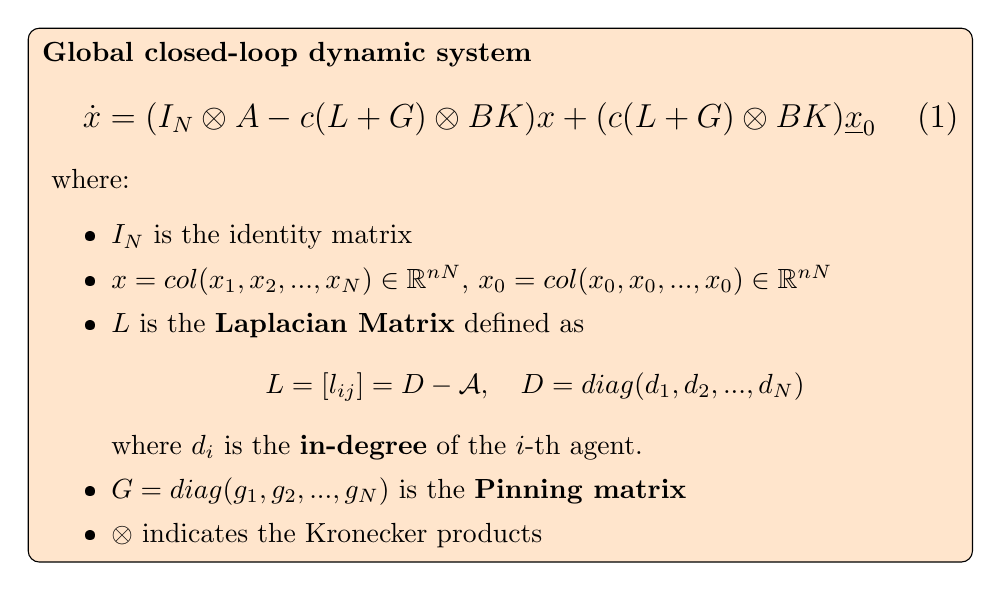
\begin{tikzpicture}
\node [mybox] (box){%
    \begin{minipage}{.96\textwidth}     
        \textbf{Global closed-loop dynamic system}
        {\large{
            \begin{equation}
                \dot{x} = (I_N \otimes A - c(L+G)\otimes BK)x +
                (c(L+G)\otimes BK)\underline{x}_{0}
            \end{equation}
        }}
        where: 
        \begin{itemize}
            \itemsep0em
            \item $I_N$ is the identity matrix
            \item $x=col(x_1,x_2,...,x_N)\in\mathbb{R}^{nN}$, $x_0=col(x_0, x_0, ..., x_0)\in\mathbb{R}^{nN}$ 
            \item $L$ is the \textbf{Laplacian Matrix} defined as \begin{equation*}
                L=[l_{ij}] = D-\mathcal{A}, \quad
                D=diag(d_1, d_2, ..., d_N) 
            \end{equation*}
            where $d_i$ is the \textbf{in-degree} of the $i$-th agent.
            \item $G=diag(g_1, g_2, ..., g_N)$ is the \textbf{Pinning matrix}
            \item $\otimes$ indicates the Kronecker products
        \end{itemize}
    \end{minipage}
};
\end{tikzpicture}%

It can be proven this results by directly applying the provided defintions and using in particular the definiton for $\otimes${
    {
    \footnote[7]{
        The \textbf{Kronecker product} is an \textbf{element-wise} operation between matrices. For example if you have 
        \begin{equation*}
            A = \begin{bmatrix}
                a_{11}&a_{12}\\a_{21}&a_{22}
            \end{bmatrix}, \ 
            B = \begin{bmatrix}
                b_{11}&b_{12}
            \end{bmatrix}
        \end{equation*}
        then $A \otimes B$ is obtained as: 
        \begin{equation*}
            A \otimes B = \begin{bmatrix}
                a_{11}B&a_{12}B\\
                a_{21}B&a_{22}B
            \end{bmatrix}=\begin{bmatrix}
                a_{11}b_{11}&a_{11}b_{12}& 
                a_{12}b_{11}&a_{12}b_{12}\\
                a_{21}b_{11}&a_{21}b_{12}& 
                a_{22}b_{11}&a_{22}b_{12}\\
            \end{bmatrix}
        \end{equation*}
    }
}
}

For the \textbf{cooperative tracking error} the objective is to track the behaviour $x_0(t)$ of the leader $S_0$, then another useful quantity related to this is the \textbf{local disagreement error} $\delta_i$ which can be extended for the overall system.\\
Then, we define as \textbf{local disagreement error} the quantity: 
\begin{equation}
    \delta_i(t) = x_i(t) - {x}_0(t)
\end{equation}
Packing together all the state variables of \textit{all the agents} the \textbf{global disagreement error} $\delta(t)$ can be defined: 
\begin{equation}
    \delta(t) = x(t)-\underline{x}_0(t)=col(\delta_1, \delta_2, \dots, \delta_N).
\end{equation}
Intuitively we can imagine that if the the \textbf{global disagreement error} is "small" in a certain sense, we reach our purpose of following the trajectory dictated by $S_0$. What is the behaviour in time of the error? This question introduces the \textbf{global disagreement dynamics} as:
\begin{align}
    &\dot{\delta_t} = \dot{x}(t) - \dot{\underline{x}}_0 = A_c \delta(t), \label{eq:GDE} \\
    &A_c = I_N \otimes A - c(L+G)\otimes BK
\end{align}
At this point the \textbf{objective of the cooperative-tracking problem} can be summarized as:
{\large{
    \begin{equation}
        \lim_{t\to\infty}  \delta(t) = 0
    \end{equation}
}}
The (\ref{eq:GDE}) is the state equation for a \textbf{dynamic system}, we know that this error \textbf{converges asymptotically to zero} if the matrix
\begin{equation*}
    A_c = I_N \otimes A - c(L+G)\otimes BK
\end{equation*}
is \textbf{Hurwitz}, i.e. all the eigenvalues $\lambda_i$ have \textbf{strictly negative real part}.\\

\noindent
\textbf{Lemma 1 (closed-loop eigenvalues)} The closed loop eigenvalues, ie the eigenvalues of $A_c$ can be computed as:
\begin{equation}
    \text{eig}(A_c) = \bigcup_{i=1}^N \text{eig}(A-c \lambda_iBK)
\end{equation}  
where $\lambda_i, \ i=1,..., N$ are the eigenvalues of the matrix $L+G$.

\section{Controller design}
\noindent
The following considerations are obtained by directly analyzing the Lemma 1:
\begin{itemize}
    \itemsep0em
    \item The \textbf{closed-loop dynamics} of the multi-agent system depends on:
    \begin{itemize}
        \item The \textbf{local controller parameters K} which are the same for each agent
         \item The eigenvalues of the matrix $L+G$ that takes into account the \textbf{communication network effect}.
        \item On the coupling gain $c$, this is used in order to cope with the communication network effect{\footnote[8]{
            In fact we will see that its value is chosen according to the $\lambda_i$s.
        }}.
    \end{itemize}
    \item The stability of the single agent does not imply the stability of the global CPS, that is
    \begin{equation*}
        (A-BK) \ \text{is Hurwitz} \nRightarrow Ac \ \text{is Hurwitz}
    \end{equation*}
\end{itemize}

\hspace*{-5mm}
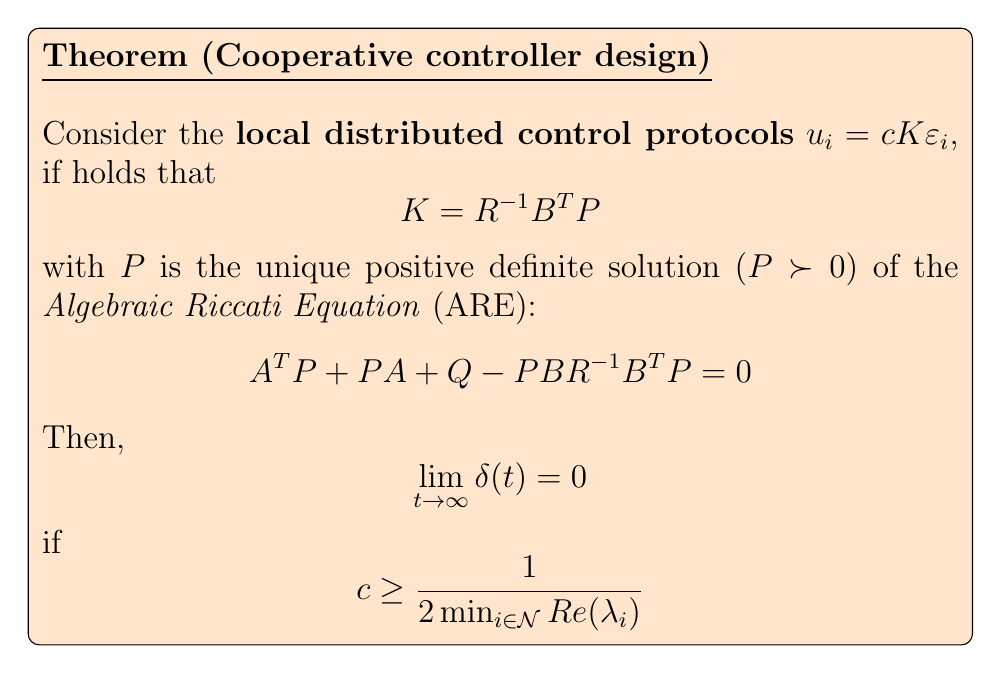
\begin{tikzpicture}
\node [mybox] (box){%
    \begin{minipage}{.96\textwidth}     
        {\large{
            \textbf{\underline{Theorem (Cooperative controller design)}}\\

            Consider the \textbf{local distributed control protocols} $u_i= c K \varepsilon_i$, if holds that
            \begin{equation*}
                K = R^{-1} B^T P
            \end{equation*}  
            with $P$ is the unique positive definite solution ($P\succ 0$) of the \textit{Algebraic Riccati Equation} (ARE):
            \begin{equation*}
                A^T P + PA + Q - PBR^{-1}B^T P = 0
            \end{equation*}
            Then,
            \begin{equation*}
                \lim_{t\to\infty} \delta(t)=0
            \end{equation*} 
            if 
            \begin{equation*}
                c \ge \frac{1} {2 \min_{i\in\mathcal{N}} Re(\lambda_i)}
            \end{equation*}
        }}
    \end{minipage}
};
\end{tikzpicture}%

\subsection{Proof of the Theorem}
In order to prove the Theorem, we need to fastly review some basic result on \textbf{optimal control} of LTI system.\\

\noindent
\textbf{Result 1 (Lyapunov equation and stability of a single LTI Equation)}
Given an LTI system described by the following equation 
\begin{equation}    \label{eq:LTI}
    \dot{x} = Ax + Bu
\end{equation}
the system is asymptotically stable (Equivalent to state that $A$ Hurwitz) if and only if the \textbf{Lyapunov Equation}
\begin{equation*}
    A^* P + PA = -Q, \ Q \succ 0
\end{equation*}
has a solution $P$ where $P$ is symmetric and definite positive $P\succ 0$. $A^*$ indicates the conjugate transpose, which in case of real matrix $A$ is $A^T$.

\subsubsection{Optimal Linear quadratic (LQ) control of LTI systems}
Let us focus on a \textbf{single LTI system} (agent) described by (\ref{eq:LTI}) and let us assume that the state is \textit{fully measured}, the objective is \textbf{compute the input $u(t)$} which solves the following optimization problem:
\begin{equation}
    \begin{aligned} \label{eq:LQ_Problem}
        u(t) = &\text{arg}\min_{u(t)} \bigg[
        \frac{1}{2} \int_0^{+\infty} {
            x^T(t)Qx(t) + u^T R u(t)
        } dt \bigg] \\
        &s.t. \\
        & \dot{x}(t) = Ax(t) + Bu(t)
    \end{aligned}
\end{equation}
The functional to be minimized is given by the \textbf{weighted sum} of the $\ell_2$-norm of the state $x(t)$ and of the input $u(t)$. \textbf{Why we want to minimize such a functional?}
\begin{itemize}
    \item By minimizing the \textbf{energy of $x(t)$}, which will be driven close to 0, we obtain: (i) shorter transient, (ii) damped oscillations; 
    \item By minimizing the \textbf{energy of} $u(t)$ we minimize the energy required from actuators.
\end{itemize}

These two issues are coupled, for this reason by choosing properly $Q, R$ we can sistematically manage the trade-off between energy of the state and command activity.\\

\noindent
\textbf{Result 2 (solution of the optimal LQ problem)}\\
The \textit{optimal solution} of the LQ problem is given by
\begin{equation}
    u(t) = -K x(t)
\end{equation}
where the matrix $K$ is given by 
\begin{equation}
    K=R^{-1} B^T P
\end{equation}
where $P \succ 0$ is the solution of the Algebraic Riccati Equation given by:
\begin{equation}
    A^T P + PA + Q + PBR^{-1}B^TP=0
\end{equation} 
\noindent
Starting from these ingredients we can demonstrate the Theorem.\\


In the \textbf{Lemma 1} we have seen that $A_c$ is Hurwitz if and only if the matrices $(A-c\lambda_i BK)$ for all $\lambda_i$, $i=1,..., N$. \\
\textbf{Under which conditions $A-c\lambda_iBK$ is Hurwitz?} From the \textbf{Result 1} we know those matrix is Hurwitz if there exits a $P\succ0$ solution of the ARE such that{
    \footnote[9]{In the next formula we use $Q_1$ in order to distinguish it from the Q used into ARE.}
}:
\begin{equation}
    (A-c\lambda_iBK)^* P + P(A-c\lambda_iBK)=-Q_1, \ Q_1 \succ 0
\end{equation}

\indent
We want to show that the left side of this equation is a symmetric positive definite matrix $Q_1$, this will be done by using simple algebraic manipulations.

\begin{align*}
    &A^T P + c\lambda_i^* K^T B^T P + PA - c\lambda_i PBK
    \overset{\text{ARE}}{=} -Q + PBR^{-1}B^T P - c\lambda_i K^T B^T P - c\lambda_iPBK =\\
    &\overset{\text{Hp:}\ K=R^{-1} B^T P}{=}
    -Q + PBR^{-1}B^TP-c\lambda_i^* (R^{-1}B^T P)^T B^T P - c \lambda_i P B R^{-1} B^T P = \\
    & = -Q + PBR^{-1} B^T P - c\lambda_i^* P B R^{-1}B^T P - c\lambda_i P B R^{-1}B^T P = \\
    & = -Q -(c(\lambda_i + \lambda_i^*)-1)P B R^{-1}B^T P \overset{\alpha_i = Re(\lambda_i)}{=} 
    - [Q+(2\alpha_i-1)P B R^{-1}B^T P]
\end{align*}

The objective is to show that $Q_1=Q+(2\alpha_i-1)P B R^{-1}B^T P$ is a symmetric positive definite matrix. But at this point we can note that: 
\begin{itemize}
    \item $Q$ is positive definite by construction; 
    \item $P$ is positive definite because it is the solution of the Algebraic Riccati Equation;
    \item $R^{-1}$ is a diagonal matrix, for this reason it is symmetric, moreover the eigenvalues (which are on the diagonal) are positive because we choose the weight ofor the input signals to be positive.
    \item Finally for any matrix $B$ even not square, the product $B^T B$ is symmetric positive definite.
\end{itemize} 
The only condition which has to be verified is that
\begin{equation}
    2c\alpha_i-1>0 \iff c>\frac{1}{2\alpha_i}=\frac{1}{2Re(\alpha_i)}
\end{equation}

\section{Dynamics of the leader $S_0$}
\noindent 
In the initial part of the discussion we have seen that the dynamics of the leader node is given by 
\begin{equation}
    \dot{x_0}(t) = A x_0(t)
\end{equation}
in which we assumed no input is applied because there is not in the discussion of the \textit{cooperative controller design}. From the basic course of dynamic systems analysis we know that the free evolution of the system $S_0$ can be computed by solving the differential equation by means of the \textbf{Laplace Transform}. In particular:
\begin{align*}
    &\dot{x}_0(t) = Ax_0(t) \iff 
    sX_0(s) - x_0(0) = A X_0(s) \iff 
    sX_0(s)-AX_0(s) = x_0(0) \iff\\
    &(sI-A)X_0(s) = x_0(0) \iff
    X_0(s) = (sI-A)^{-1} x_0(0)  
\end{align*}
By applying the \textit{inverse Laplace transform} we can say that
\begin{equation}
    X_0(s) \overset{\mathcal{L}^{-1}}{\iff} x_0(t) = \mathcal{L}^{-1} \{
        (sI-A)^{-1} x_0(0)
    \}
\end{equation}
From this equation we observe that in order to get something interesting from the dynamics of the system we need some initial conditions. However, it is not said that the natural modes of the system satisfy us, that is the free evolution of the system does not satisfy the trajectory we want to dictate. \textbf{How ca we force the leader to generate a certain trajectory?} We have to modify the dynamics of the leader by modifying the eigenvalues of the matrix $A$ by using the pole placement technique. For example: 
\begin{enumerate}
    \item If we want the leader to generate a \textbf{step} we need an eigenvalue equal to zero and the remaining part of the eigenvalues to be with negative real part.
    \item If we want a \textbf{ramp} we need two coincident eigenvalues and remaining part to be stable.
    \item For a \textbf{sinusoidal reference} you need to manipulate with magnitude and phase of \textbf{complex conjugate eigenvalues}.
\end{enumerate}

Remember that these results come from the modal analysis and from the resulting Partial Fraction Decomposition (PFE) of the Laplace transform for the system under discussion.\\

If nothing is modified the cooperative control protocol applied to each agent does not permit to reach the tracking as desired. Why? We have assumed the matrices $(A,B,C)$ to be equal for all the agents. Changing the dynamic matrix $A$ for the leader, also the followers have to change. For this reason:
\begin{itemize}
    \item We have to know which trajectory is desired for the agent to follow, and according to this deciding the \textbf{eigenvalues};
    \item The matrix $K$ is decided accordingly
    \item This matrix will modify also the matrices of the dynamics for the agents in a way that applying the \textbf{cooperative control protocol} all can work fine.
\end{itemize}



\chapter{Cooperative dynamic-regulator for synchronization of multi-agent sytems}
In the previous chapter we have assumed that the state was fully measurable, i.e. the matrix $C=I$. This hypotesis in general does not hold for real world applications and so in order to design a \textit{cooperative control system} we first need to \textbf{estimate the state} $x_i$ of each agent. \\
This is the reason that leads us to design a \textbf{design a device} which provides an \textbf{estimate} $\hat{x}_i$ of the state $x_i$ \textbf{for each agent} such that 
\begin{equation}
    \lim_{t \to \infty} \hat{x}(t) = x(t)
\end{equation}

\section{Cooperative observer design for a single agent}
The only information can be shared among the agents is the \textbf{local output estimation error} which is defined as
\begin{equation}
    \tilde{y}_i = y_i - \hat{y}_i = y_i - C \hat{x}_i 
\end{equation}
For the design of the \textbf{local observer} is important also another quantity that is the \textbf{neighbourhood output estimation error} which is defined as: 
{\large
    \begin{equation}
        \xi_i = \sum_{j=1}^N {a_{ij} (\tilde{y}_j - \tilde{y}_i) + g_i(\tilde{y}_0 - \tilde{y}_i)}
    \end{equation}
}
Finally for a single agent in a cooperative context, the \textbf{cooperative observer} is by 
\begin{equation} \label{eq: coop_OBSV}
    \dot{\hat{x}}_i = A \hat{x}_i + B u_i - cF\xi_i
\end{equation}
This cooperative protocol leads to a \textbf{completely distributed observer} in the sense that is based only on: 
\begin{itemize}
    \item The \textbf{local output estimation error} $\tilde{y}_i$
    \item The \textbf{estimation error} of the neighbours which is expressed by the succint number $\xi_i$
\end{itemize} 

\section{Global estimation error and global observer}
We can pack together the equations for the local cooperative observers in order to obtain a \textbf{global cooperative observer dynamics}, defined as:
\begin{equation}
    \dot{\hat{x}}= A_o\hat{x} + 
    (I_N \otimes B) u + c ((L+G)\otimes F) y
\end{equation}
where:
\begin{itemize}
    \item $A_o= (I_N \otimes A) - c ((L+G)\otimes FC)$
    \item $\hat{x} = col(\hat{x_1}, \hat{x_2}, ..., \hat{x_N})$, \quad $u=col(u_1, u_2, ..., u_N)$ \quad $y=col(y_1,y_2, ..., y_N)$
\end{itemize}
\noindent
The \textbf{global state estimation error} is defined as: 
\begin{equation}
    \tilde{x}(t) = x(t)-\hat{x}(t)
\end{equation}
where $x(t) = col(x_1(t), x_2(t), ..., x_N(t))$ and $\hat{x} = col(\hat{x_1}, \hat{x_2}, ..., \hat{x_N})$. 
As in the case of the controller design we are interested in make this error as close as possible to zero. So one can wonder what is its evolution in time. We consider at this aim the \textbf{global estimation error dynamics} which is defined as: 
\begin{equation}  \label{eq:GEED}
    \dot{\tilde{x}}(t) = \dot{x}_i(t) - \dot{\hat{x}}_i(t) = A_o \tilde{x}(t)
\end{equation}
Our objective here is that
\begin{equation}
    \lim_{t\to\infty} \tilde{x}(t) = 0; 
\end{equation}
Since the equation (\ref{eq:GEED}) represents the state equation for a dynamic system, then this system (representing the evolution of the global estimation error in time) will converge to zero (i.e. it is asymptotically stable) if the matrix $A_o$ defined as:
\begin{equation}
    A_o=(I_N \otimes A) - c ((L+G)\otimes FC)
\end{equation} 
is \textbf{Hurwitz}.

\subsection{Global observer eigenvalues and design}
The eigenvalues of the \textbf{global observer} are given by the following Lemma. 

\noindent
\textbf{Lemma 2(global observer eigenvalues)} The eigenvalues of the global observer are given by
\begin{equation*}
    eig(A_o) = \bigcup_{i=1}^N eig(A-c\lambda_i FC) 
\end{equation*}
where $\lambda_i$ are the eigenvalues of the matrix $L+G$.
The following theorem provides us with a tool by which the value for $c$, $F$ can be choosen in order to implement a \textbf{global observer}.\\

%Per disegnare il box
\hspace*{-5mm}
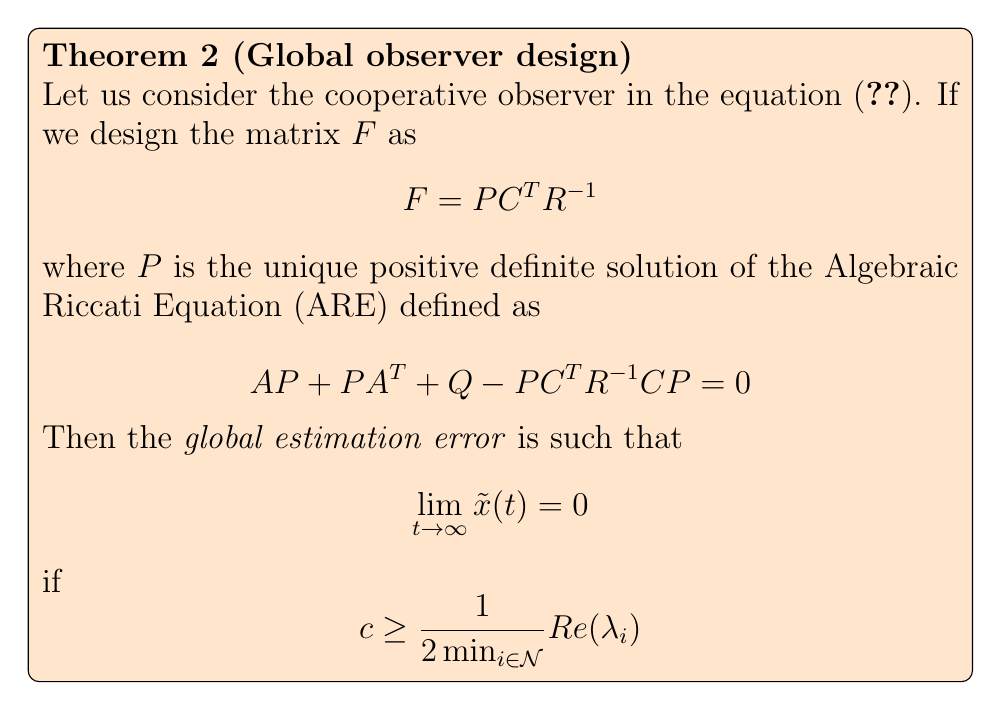
\begin{tikzpicture}
\node [mybox] (box){%
    \begin{minipage}{.96\textwidth}    
        {\large{
            \textbf{Theorem 2 (Global observer design)}\\
            Let us consider the cooperative observer in the equation (\ref{eq: coop_OBSV}). If we design the matrix $F$ as 
            \begin{equation*}
                F = P C^T R^{-1}
            \end{equation*}
            where $P$ is the unique positive definite solution of the Algebraic Riccati Equation (ARE) defined as
        
            \begin{equation*}
                AP + PA^T + Q - P C^T R^{-1} C P = 0
            \end{equation*}
            Then the \textit{global estimation error} is such that
            \begin{equation*}
                \lim_{t\to\infty} \tilde{x}(t)=0
            \end{equation*} if 
            \begin{equation*}
                c \ge \frac{1}{2 \min_{i\in \mathcal{N}}} Re(\lambda_i)
            \end{equation*}
        }}
    \end{minipage}
};
\end{tikzpicture}%

\section{Cooperative dynamic regulator design}
\noindent
We know that for an LTI system that is fully observable and fully controllable we can design a device, the so-called dynamic regulator made up of a controller and an observer. The interesting thing here is that, while in the case of a single agent there is a unique way to design the dynamic regulator, when we have a multi-agent system there are several way to build such a device, three in particular:
\begin{enumerate}
    \item Neighbourhood observer and neighbourhood controller
    \item Local observer and neighbourhood controller
    \item Local observer and local controller
\end{enumerate}
We will the first two cases since are the most interesting.

\subsection{\color{red}1st approach: Neighbourhood controller and neighbourhood observer}
In this case we can build the dynamic regulator by design: 
\begin{enumerate}
    \item A state variables feedback \underline{\textbf{(SVFB) distributed control protocol}}
    \begin{equation*}
        u_i = cK\hat{\varepsilon}_i
    \end{equation*}
    where $\hat{\varepsilon}_i$ is the \textit{local neighbourhood state estimation error} and it is defined as 
    \begin{equation*}
        \hat{\varepsilon}_i = \sum_{j=1}^N a_{ij} (\hat{x_j}-\hat{x_i}) + g_i (\hat{x}_0 - \hat{x}_i)
    \end{equation*}
    \item A \textbf{\underline{cooperative distributed observer}} with dynamics
    \begin{equation*}
        \dot{\hat{x}}_i = A \hat{x_i} + B u_i - cF\xi_i
    \end{equation*}
    where the term $\xi_i$ is the \textit{local neighbourhood output estimation error} defined as before.
\end{enumerate}

\noindent
At this point the \textbf{local closed-dynamics} is defined by the pair:
\begin{align*}
    &\dot{x}_i = Ax_i + c B K \biggl(
        \sum_{j=1}^N a_{ij} (\hat{x_j}-\hat{x_i}) + g_i (\hat{x}_0 - \hat{x}_i)
    \biggr)\\
    &\dot{\hat{x}}_i = A \hat{x_i} + B u_i -cF\biggl(
        \sum_{i=1}^N a_{ij} (\tilde{y}_j - \tilde{y}_i) + g_i (\tilde{y}_0 - \tilde{y}_i)
    \biggr)
\end{align*}
Following the path of the previous chapters, by choosing as state variables the \textbf{global disagreement error} and the \textbf{global estimation error}, the  \textbf{global closed-loop dynamics} is the following: 
{\large{
    \begin{equation*}
        \begin{bmatrix}
            \dot{\delta}\\\dot{\tilde{x}} 
        \end{bmatrix} = \begin{bmatrix}
            A_c&B_c\\
            0&A_o
        \end{bmatrix}
        \begin{bmatrix}
            \delta\\\tilde{x}
        \end{bmatrix}
    \end{equation*}
}}

The result which has just exposed states that the \textit{global disagreement error dynamics} depends only on $c$ and $K$ no matter if the state variables are measurable or not, moreover the \textit{global estimation error dynamics} depends only on $c$ and $F$ without taking into account if an SVFB or another protocol has been used. This important property is the so-called \textbf{separation principle}.

\subsection{\color{red}2nd approach: Neighbourhood controller and local observer}
There is an alternative way to design a cooperative distributed dynamic regulator, which is keeping the SVFB protocol in order to design $c$, $K$ in order to get the agents tracking the leader. The novelty here is that locally, for each agent, it is used a \textbf{local observer} instead of a \textbf{cooperative observer}, its dynamics is given by
\begin{equation*}
    \dot{\hat{x}}_i = A \hat{x}_i + B ui - cF\tilde{y}_i
\end{equation*}
where $\tilde{y}_i$ is the \textbf{local output estimation error}. In the previous paragraph we have seen that insted of this quantity the information from the neighbourhood was exploited to build a cooperative observer.
Even in this case we can define a \textbf{global closed-loop  dynamics} as
{\large{
    \begin{equation*}
        \begin{bmatrix}
            \dot{\delta}\\
            \dot{\tilde{x}}
        \end{bmatrix} = \begin{bmatrix}
            A_c& B_c\\
            0&(I \otimes (A+cFC))
        \end{bmatrix} \begin{bmatrix}
            \delta\\
            \tilde{x}
        \end{bmatrix}
    \end{equation*}
}}
In this case the global observer eigenvalues are obtained by putting together the eigen values of the matrix $(A+cFC)$ for each agent from 1 to N. This states that it sufficient to properly design $F$ in order to drive the (global) estimation error to 0. 


\section{Example of Cooperative tracking control }
\noindent
Let's consider a multi-agent system where each single agent $S_i$ is described as follows 

\begin{figure}[h]
    \centering
    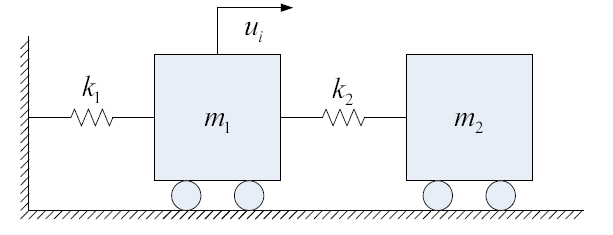
\includegraphics[scale=0.7]{images/excoop.png}
\end{figure}
\noindent
Each agent can be modeled as follows: 
\begin{equation*}
    \begin{aligned}
        &\dot{x}_i = A x_i + B u_i\\
        &y = Cx_i
    \end{aligned}
\end{equation*}

where $x_i = [p_1^i, \ v_1^i, \  p_2^i, \ v_2^i]^T$ where $p_1, p_2$ are the \textit{displacement} with respect to the position \textbf{at rest}. The input $u_i$ is a force applied to the mass $m_1$ of each agent $S_i$. The values for the parameters are: $m_1 = 1.1 \ kg$, $m_2 = 0.9 \ kg$, $K_1 = 1.5 \ N/m$, $K_2 = 1 \ N/m$. Note that \textbf{the leader node is unforced} that is $u_0=0$.

The multi-agent system is made up of a \textbf{leader node} and \textbf{six follower nodes} which are interconnected following the graph in the figure below

\begin{figure}[h]
    \centering
    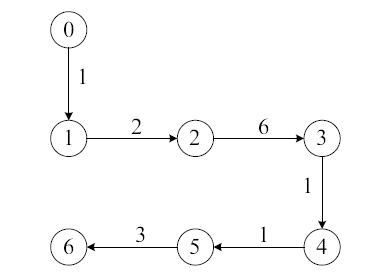
\includegraphics[scale=1]{images/graphTop.png}
\end{figure}

The objective here is to design a global cooperative tracking controller in order to follow the trajectory dictated by the leader node which is producing a desired trajectory. Let's assume randomly generated values for the initial conditions for all the state variables $x_i$.\\
As further step you can consider that the state is not fully measurable and to build a cooperative controller following the two proposed approaches  and then by using such an estimate to design a SVFB protocol. In other words the additive task is to design a \textit{cooperative distributed dynamic regulator}. In order to carry out this task you can assume (in a quite realistic way) that only positions are measurable, the resulting matrix $C$ to be used is the following: 
\begin{equation*}
    C = \begin{bmatrix}
        1&0&0&0\\
        0&0&1&0
    \end{bmatrix}
\end{equation*}







\chapter{Formation control}


\end{document}
